\documentclass{book}
\usepackage[a4paper,top=2.5cm,bottom=2.5cm,left=2.5cm,right=2.5cm]{geometry}
\usepackage{makeidx}
\usepackage{natbib}
\usepackage{graphicx}
\usepackage{multicol}
\usepackage{float}
\usepackage{listings}
\usepackage{color}
\usepackage{ifthen}
\usepackage[table]{xcolor}
\usepackage{textcomp}
\usepackage{alltt}
\usepackage{ifpdf}
\ifpdf
\usepackage[pdftex,
            pagebackref=true,
            colorlinks=true,
            linkcolor=blue,
            unicode
           ]{hyperref}
\else
\usepackage[ps2pdf,
            pagebackref=true,
            colorlinks=true,
            linkcolor=blue,
            unicode
           ]{hyperref}
\usepackage{pspicture}
\fi
\usepackage[utf8]{inputenc}
\usepackage[french]{babel}

\usepackage{mathptmx}
\usepackage[scaled=.90]{helvet}
\usepackage{courier}
\usepackage{sectsty}
\usepackage{amssymb}
\usepackage[titles]{tocloft}
\usepackage{doxygen}
\lstset{language=C++,inputencoding=utf8,basicstyle=\footnotesize,breaklines=true,breakatwhitespace=true,tabsize=8,numbers=left }
\makeindex
\setcounter{tocdepth}{3}
\renewcommand{\footrulewidth}{0.4pt}
\renewcommand{\familydefault}{\sfdefault}
\hfuzz=15pt
\setlength{\emergencystretch}{15pt}
\hbadness=750
\tolerance=750
\begin{document}
\hypersetup{pageanchor=false,citecolor=blue}
\begin{titlepage}
\vspace*{7cm}
\begin{center}
{\Large G\-S\-B\-\_\-\-Appli }\\
\vspace*{1cm}
{\large Généré par Doxygen 1.8.1.2}\\
\vspace*{0.5cm}
{\small Mardi Décembre 10 2013 23:18:41}\\
\end{center}
\end{titlepage}
\clearemptydoublepage
\pagenumbering{roman}
\tableofcontents
\clearemptydoublepage
\pagenumbering{arabic}
\hypersetup{pageanchor=true,citecolor=blue}
\chapter{Liste des choses à faire}
\label{todo}
\hypertarget{todo}{}

\begin{DoxyRefList}
\item[\label{todo__todo000001}%
\hypertarget{todo__todo000001}{}%
Espace de nommage \hyperlink{namespacedefault}{default} ]R\-A\-S 

R\-A\-S 

R\-A\-S 

R\-A\-S 

R\-A\-S 

Fonctions retournant plusieurs lignes sont à réécrire. 

R\-A\-S 

R\-A\-S 

R\-A\-S 

fonction est\-Mois\-Valide à définir complètement ou à supprimer 
\end{DoxyRefList}
\chapter{Index des espaces de nommage}
\section{Liste des espaces de nommage}
Liste de tous les espaces de nommage avec une brève description\-:\begin{DoxyCompactList}
\item\contentsline{section}{\hyperlink{namespacedefault}{default} }{\pageref{namespacedefault}}{}
\end{DoxyCompactList}

\chapter{Index des fichiers}
\section{Liste des fichiers}
Liste de tous les fichiers avec une brève description \-:\begin{DoxyCompactList}
\item\contentsline{section}{/home/trackoen/\-P\-H\-P\-\_\-\-P\-R\-O\-J\-E\-C\-T/\-G\-S\-B\-\_\-\-Appli/\hyperlink{c_accueil_8php}{c\-Accueil.\-php} }{\pageref{c_accueil_8php}}{}
\item\contentsline{section}{/home/trackoen/\-P\-H\-P\-\_\-\-P\-R\-O\-J\-E\-C\-T/\-G\-S\-B\-\_\-\-Appli/\hyperlink{c_consult_fiches_frais_8php}{c\-Consult\-Fiches\-Frais.\-php} }{\pageref{c_consult_fiches_frais_8php}}{}
\item\contentsline{section}{/home/trackoen/\-P\-H\-P\-\_\-\-P\-R\-O\-J\-E\-C\-T/\-G\-S\-B\-\_\-\-Appli/\hyperlink{c_saisie_fiche_frais_8php}{c\-Saisie\-Fiche\-Frais.\-php} }{\pageref{c_saisie_fiche_frais_8php}}{}
\item\contentsline{section}{/home/trackoen/\-P\-H\-P\-\_\-\-P\-R\-O\-J\-E\-C\-T/\-G\-S\-B\-\_\-\-Appli/\hyperlink{c_se_connecter_8php}{c\-Se\-Connecter.\-php} }{\pageref{c_se_connecter_8php}}{}
\item\contentsline{section}{/home/trackoen/\-P\-H\-P\-\_\-\-P\-R\-O\-J\-E\-C\-T/\-G\-S\-B\-\_\-\-Appli/\hyperlink{c_se_deconnecter_8php}{c\-Se\-Deconnecter.\-php} }{\pageref{c_se_deconnecter_8php}}{}
\item\contentsline{section}{/home/trackoen/\-P\-H\-P\-\_\-\-P\-R\-O\-J\-E\-C\-T/\-G\-S\-B\-\_\-\-Appli/\hyperlink{maj_g_s_b__main_8php}{maj\-G\-S\-B\-\_\-main.\-php} }{\pageref{maj_g_s_b__main_8php}}{}
\item\contentsline{section}{/home/trackoen/\-P\-H\-P\-\_\-\-P\-R\-O\-J\-E\-C\-T/\-G\-S\-B\-\_\-\-Appli/include/\hyperlink{__bd_gestion_donnees_8lib_8php}{\-\_\-bd\-Gestion\-Donnees.\-lib.\-php} }{\pageref{__bd_gestion_donnees_8lib_8php}}{}
\item\contentsline{section}{/home/trackoen/\-P\-H\-P\-\_\-\-P\-R\-O\-J\-E\-C\-T/\-G\-S\-B\-\_\-\-Appli/include/\hyperlink{__fin_8inc_8php}{\-\_\-fin.\-inc.\-php} }{\pageref{__fin_8inc_8php}}{}
\item\contentsline{section}{/home/trackoen/\-P\-H\-P\-\_\-\-P\-R\-O\-J\-E\-C\-T/\-G\-S\-B\-\_\-\-Appli/include/\hyperlink{__gestion_session_8lib_8php}{\-\_\-gestion\-Session.\-lib.\-php} }{\pageref{__gestion_session_8lib_8php}}{}
\item\contentsline{section}{/home/trackoen/\-P\-H\-P\-\_\-\-P\-R\-O\-J\-E\-C\-T/\-G\-S\-B\-\_\-\-Appli/include/\hyperlink{__init_8inc_8php}{\-\_\-init.\-inc.\-php} }{\pageref{__init_8inc_8php}}{}
\item\contentsline{section}{/home/trackoen/\-P\-H\-P\-\_\-\-P\-R\-O\-J\-E\-C\-T/\-G\-S\-B\-\_\-\-Appli/include/\hyperlink{__sommaire_8inc_8php}{\-\_\-sommaire.\-inc.\-php} }{\pageref{__sommaire_8inc_8php}}{}
\item\contentsline{section}{/home/trackoen/\-P\-H\-P\-\_\-\-P\-R\-O\-J\-E\-C\-T/\-G\-S\-B\-\_\-\-Appli/include/\hyperlink{__utilitaires_et_gestion_erreurs_8lib_8php}{\-\_\-utilitaires\-Et\-Gestion\-Erreurs.\-lib.\-php} }{\pageref{__utilitaires_et_gestion_erreurs_8lib_8php}}{}
\item\contentsline{section}{/home/trackoen/\-P\-H\-P\-\_\-\-P\-R\-O\-J\-E\-C\-T/\-G\-S\-B\-\_\-\-Appli/include/\hyperlink{fct_8inc_8php}{fct.\-inc.\-php} }{\pageref{fct_8inc_8php}}{}
\end{DoxyCompactList}

\chapter{Documentation des espaces de nommage}
\hypertarget{namespacedefault}{\section{Référence de l'espace de nommage default}
\label{namespacedefault}\index{default@{default}}
}


\subsection{Description détaillée}
Page d'accueil de l'application web Appli\-Frais

\begin{DoxyRefDesc}{A faire}
\item[\hyperlink{todo__todo000001}{A faire}]R\-A\-S \end{DoxyRefDesc}


Script de contrôle et d'affichage du cas d'utilisation \char`\"{}\-Consulter une fiche de frais\char`\"{}

\begin{DoxyRefDesc}{A faire}
\item[\hyperlink{todo__todo000002}{A faire}]R\-A\-S \end{DoxyRefDesc}


Script de contrôle et d'affichage du cas d'utilisation \char`\"{}\-Saisir fiche de frais\char`\"{}

\begin{DoxyRefDesc}{A faire}
\item[\hyperlink{todo__todo000003}{A faire}]R\-A\-S \end{DoxyRefDesc}


Script de contrôle et d'affichage du cas d'utilisation \char`\"{}\-Se connecter\char`\"{}

\begin{DoxyRefDesc}{A faire}
\item[\hyperlink{todo__todo000004}{A faire}]R\-A\-S \end{DoxyRefDesc}


Script de contrôle et d'affichage du cas d'utilisation \char`\"{}\-Se déconnecter\char`\"{}

\begin{DoxyRefDesc}{A faire}
\item[\hyperlink{todo__todo000005}{A faire}]R\-A\-S \end{DoxyRefDesc}


Regroupe les fonctions d'accès aux données.

\begin{DoxyAuthor}{Auteur}
Arthur Martin 
\end{DoxyAuthor}
\begin{DoxyRefDesc}{A faire}
\item[\hyperlink{todo__todo000006}{A faire}]Fonctions retournant plusieurs lignes sont à réécrire. \end{DoxyRefDesc}


Libère les ressources nécessaires au fonctionnement de l'application

\begin{DoxyRefDesc}{A faire}
\item[\hyperlink{todo__todo000007}{A faire}]R\-A\-S \end{DoxyRefDesc}


Regroupe les fonctions de gestion d'une session utilisateur.

\begin{DoxyRefDesc}{A faire}
\item[\hyperlink{todo__todo000008}{A faire}]R\-A\-S \end{DoxyRefDesc}


Initialise les ressources nécessaires au fonctionnement de l'application

\begin{DoxyRefDesc}{A faire}
\item[\hyperlink{todo__todo000009}{A faire}]R\-A\-S \end{DoxyRefDesc}


Regroupe les fonctions utilitaires et de gestion des erreurs.

\begin{DoxyRefDesc}{A faire}
\item[\hyperlink{todo__todo000011}{A faire}]fonction est\-Mois\-Valide à définir complètement ou à supprimer \end{DoxyRefDesc}

\chapter{Documentation des fichiers}
\hypertarget{c_accueil_8php}{\section{Référence du fichier /home/trackoen/\-P\-H\-P\-\_\-\-P\-R\-O\-J\-E\-C\-T/\-G\-S\-B\-\_\-\-Appli/c\-Accueil.php}
\label{c_accueil_8php}\index{/home/trackoen/\-P\-H\-P\-\_\-\-P\-R\-O\-J\-E\-C\-T/\-G\-S\-B\-\_\-\-Appli/c\-Accueil.\-php@{/home/trackoen/\-P\-H\-P\-\_\-\-P\-R\-O\-J\-E\-C\-T/\-G\-S\-B\-\_\-\-Appli/c\-Accueil.\-php}}
}
\subsection*{Espaces de nommage}
\begin{DoxyCompactItemize}
\item 
namespace \hyperlink{namespacedefault}{default}
\end{DoxyCompactItemize}
\subsection*{Variables}
\begin{DoxyCompactItemize}
\item 
\hyperlink{c_accueil_8php_aad2a80747c2de66b59cb18d493ae7a8b}{\$rep\-Include} = './include/'
\item 
\hyperlink{c_accueil_8php_a5b407bc19b08452156cf04e24ef10ed7}{if} (!\hyperlink{__gestion_session_8lib_8php_afe911e51f16958708b8b700981cd2567}{est\-Visiteur\-Connecte}())
\end{DoxyCompactItemize}


\subsection{Documentation des variables}
\hypertarget{c_accueil_8php_aad2a80747c2de66b59cb18d493ae7a8b}{\index{c\-Accueil.\-php@{c\-Accueil.\-php}!\$rep\-Include@{\$rep\-Include}}
\index{\$rep\-Include@{\$rep\-Include}!cAccueil.php@{c\-Accueil.\-php}}
\subsubsection[{\$rep\-Include}]{\setlength{\rightskip}{0pt plus 5cm}\$rep\-Include = './include/'}}\label{c_accueil_8php_aad2a80747c2de66b59cb18d493ae7a8b}


Définition à la ligne 7 du fichier c\-Accueil.\-php.

\hypertarget{c_accueil_8php_a5b407bc19b08452156cf04e24ef10ed7}{\index{c\-Accueil.\-php@{c\-Accueil.\-php}!if@{if}}
\index{if@{if}!cAccueil.php@{c\-Accueil.\-php}}
\subsubsection[{if}]{\setlength{\rightskip}{0pt plus 5cm}if(!{\bf est\-Visiteur\-Connecte}())}}\label{c_accueil_8php_a5b407bc19b08452156cf04e24ef10ed7}


Définition à la ligne 11 du fichier c\-Accueil.\-php.


\hypertarget{c_consult_fiches_frais_8php}{\section{Référence du fichier /home/trackoen/\-P\-H\-P\-\_\-\-P\-R\-O\-J\-E\-C\-T/\-G\-S\-B\-\_\-\-Appli/c\-Consult\-Fiches\-Frais.php}
\label{c_consult_fiches_frais_8php}\index{/home/trackoen/\-P\-H\-P\-\_\-\-P\-R\-O\-J\-E\-C\-T/\-G\-S\-B\-\_\-\-Appli/c\-Consult\-Fiches\-Frais.\-php@{/home/trackoen/\-P\-H\-P\-\_\-\-P\-R\-O\-J\-E\-C\-T/\-G\-S\-B\-\_\-\-Appli/c\-Consult\-Fiches\-Frais.\-php}}
}
\subsection*{Espaces de nommage}
\begin{DoxyCompactItemize}
\item 
namespace \hyperlink{namespacedefault}{default}
\end{DoxyCompactItemize}
\subsection*{Variables}
\begin{DoxyCompactItemize}
\item 
\hyperlink{c_consult_fiches_frais_8php_aad2a80747c2de66b59cb18d493ae7a8b}{\$rep\-Include} = './include/'
\item 
\hyperlink{c_consult_fiches_frais_8php_a12d9ecce0abd3757dd699cc19040e747}{if} (!\hyperlink{__gestion_session_8lib_8php_afe911e51f16958708b8b700981cd2567}{est\-Visiteur\-Connecte}())
\item 
\hyperlink{c_consult_fiches_frais_8php_aca0267343316d569312879584a4db9dd}{\$mois\-Saisi} = \hyperlink{__utilitaires_et_gestion_erreurs_8lib_8php_ab0070fc1ef4283caa3457dd5b71a86de}{lire\-Donnee\-Post}(\char`\"{}lst\-Mois\char`\"{}, \char`\"{}\char`\"{})
\item 
\hyperlink{c_consult_fiches_frais_8php_a5c1bc42ba293d577d9e25d76e50f85ec}{\$etape} = \hyperlink{__utilitaires_et_gestion_erreurs_8lib_8php_ab0070fc1ef4283caa3457dd5b71a86de}{lire\-Donnee\-Post}(\char`\"{}etape\char`\"{},\char`\"{}\char`\"{})
\item 
\hyperlink{c_se_connecter_8php_a161e098d41499c163a94c3fa5cd0e698}{if}(\$etape!=\char`\"{}demander\-Consult\char`\"{}\&\&\$etape!=\char`\"{}valider\-Consult\char`\"{}) \\*
if(\$etape==\char`\"{}valider\-Consult\char`\"{}) \hyperlink{c_consult_fiches_frais_8php_aa8307f98fa28d7f64c9762e7986440b6}{\$req} = \hyperlink{__bd_gestion_donnees_8lib_8php_af7ab441030c5c590de0b463414880a16}{obtenir\-Req\-Mois\-Fiche\-Frais}(\hyperlink{__gestion_session_8lib_8php_a7af627b049f30bda0af2678c3327aff0}{obtenir\-Id\-User\-Connecte}())
\item 
\hyperlink{c_consult_fiches_frais_8php_ae3f221921bd93ca690a99b756043483c}{\$id\-Jeu\-Mois} = mysql\-\_\-query(\$req, \$id\-Connexion)
\item 
\hyperlink{c_consult_fiches_frais_8php_ad97348117c6ea6767b8494f27a153a0f}{\$lg\-Mois} = mysql\-\_\-fetch\-\_\-assoc(\$id\-Jeu\-Mois)
\end{DoxyCompactItemize}


\subsection{Documentation des variables}
\hypertarget{c_consult_fiches_frais_8php_a5c1bc42ba293d577d9e25d76e50f85ec}{\index{c\-Consult\-Fiches\-Frais.\-php@{c\-Consult\-Fiches\-Frais.\-php}!\$etape@{\$etape}}
\index{\$etape@{\$etape}!cConsultFichesFrais.php@{c\-Consult\-Fiches\-Frais.\-php}}
\subsubsection[{\$etape}]{\setlength{\rightskip}{0pt plus 5cm}\$etape = {\bf lire\-Donnee\-Post}(\char`\"{}etape\char`\"{},\char`\"{}\char`\"{})}}\label{c_consult_fiches_frais_8php_a5c1bc42ba293d577d9e25d76e50f85ec}


Définition à la ligne 19 du fichier c\-Consult\-Fiches\-Frais.\-php.

\hypertarget{c_consult_fiches_frais_8php_ae3f221921bd93ca690a99b756043483c}{\index{c\-Consult\-Fiches\-Frais.\-php@{c\-Consult\-Fiches\-Frais.\-php}!\$id\-Jeu\-Mois@{\$id\-Jeu\-Mois}}
\index{\$id\-Jeu\-Mois@{\$id\-Jeu\-Mois}!cConsultFichesFrais.php@{c\-Consult\-Fiches\-Frais.\-php}}
\subsubsection[{\$id\-Jeu\-Mois}]{\setlength{\rightskip}{0pt plus 5cm}\$id\-Jeu\-Mois = mysql\-\_\-query(\$req, \$id\-Connexion)}}\label{c_consult_fiches_frais_8php_ae3f221921bd93ca690a99b756043483c}


Définition à la ligne 52 du fichier c\-Consult\-Fiches\-Frais.\-php.

\hypertarget{c_consult_fiches_frais_8php_ad97348117c6ea6767b8494f27a153a0f}{\index{c\-Consult\-Fiches\-Frais.\-php@{c\-Consult\-Fiches\-Frais.\-php}!\$lg\-Mois@{\$lg\-Mois}}
\index{\$lg\-Mois@{\$lg\-Mois}!cConsultFichesFrais.php@{c\-Consult\-Fiches\-Frais.\-php}}
\subsubsection[{\$lg\-Mois}]{\setlength{\rightskip}{0pt plus 5cm}\$lg\-Mois = mysql\-\_\-fetch\-\_\-assoc(\$id\-Jeu\-Mois)}}\label{c_consult_fiches_frais_8php_ad97348117c6ea6767b8494f27a153a0f}


Définition à la ligne 53 du fichier c\-Consult\-Fiches\-Frais.\-php.

\hypertarget{c_consult_fiches_frais_8php_aca0267343316d569312879584a4db9dd}{\index{c\-Consult\-Fiches\-Frais.\-php@{c\-Consult\-Fiches\-Frais.\-php}!\$mois\-Saisi@{\$mois\-Saisi}}
\index{\$mois\-Saisi@{\$mois\-Saisi}!cConsultFichesFrais.php@{c\-Consult\-Fiches\-Frais.\-php}}
\subsubsection[{\$mois\-Saisi}]{\setlength{\rightskip}{0pt plus 5cm}\$mois\-Saisi = {\bf lire\-Donnee\-Post}(\char`\"{}lst\-Mois\char`\"{}, \char`\"{}\char`\"{})}}\label{c_consult_fiches_frais_8php_aca0267343316d569312879584a4db9dd}


Définition à la ligne 18 du fichier c\-Consult\-Fiches\-Frais.\-php.

\hypertarget{c_consult_fiches_frais_8php_aad2a80747c2de66b59cb18d493ae7a8b}{\index{c\-Consult\-Fiches\-Frais.\-php@{c\-Consult\-Fiches\-Frais.\-php}!\$rep\-Include@{\$rep\-Include}}
\index{\$rep\-Include@{\$rep\-Include}!cConsultFichesFrais.php@{c\-Consult\-Fiches\-Frais.\-php}}
\subsubsection[{\$rep\-Include}]{\setlength{\rightskip}{0pt plus 5cm}\$rep\-Include = './include/'}}\label{c_consult_fiches_frais_8php_aad2a80747c2de66b59cb18d493ae7a8b}


Définition à la ligne 7 du fichier c\-Consult\-Fiches\-Frais.\-php.

\hypertarget{c_consult_fiches_frais_8php_aa8307f98fa28d7f64c9762e7986440b6}{\index{c\-Consult\-Fiches\-Frais.\-php@{c\-Consult\-Fiches\-Frais.\-php}!\$req@{\$req}}
\index{\$req@{\$req}!cConsultFichesFrais.php@{c\-Consult\-Fiches\-Frais.\-php}}
\subsubsection[{\$req}]{\setlength{\rightskip}{0pt plus 5cm}{\bf if} (\$etape!=\char`\"{}demander\-Consult\char`\"{}\&\&\$etape!=\char`\"{}valider\-Consult\char`\"{}) if (\$etape==\char`\"{}valider\-Consult\char`\"{}) \$req = {\bf obtenir\-Req\-Mois\-Fiche\-Frais}({\bf obtenir\-Id\-User\-Connecte}())}}\label{c_consult_fiches_frais_8php_aa8307f98fa28d7f64c9762e7986440b6}


Définition à la ligne 51 du fichier c\-Consult\-Fiches\-Frais.\-php.

\hypertarget{c_consult_fiches_frais_8php_a12d9ecce0abd3757dd699cc19040e747}{\index{c\-Consult\-Fiches\-Frais.\-php@{c\-Consult\-Fiches\-Frais.\-php}!if@{if}}
\index{if@{if}!cConsultFichesFrais.php@{c\-Consult\-Fiches\-Frais.\-php}}
\subsubsection[{if}]{\setlength{\rightskip}{0pt plus 5cm}if(\$etape==\char`\"{}valider\-Consult\char`\"{})}}\label{c_consult_fiches_frais_8php_a12d9ecce0abd3757dd699cc19040e747}


Définition à la ligne 11 du fichier c\-Consult\-Fiches\-Frais.\-php.


\hypertarget{c_saisie_fiche_frais_8php}{\section{Référence du fichier /home/trackoen/\-P\-H\-P\-\_\-\-P\-R\-O\-J\-E\-C\-T/\-G\-S\-B\-\_\-\-Appli/c\-Saisie\-Fiche\-Frais.php}
\label{c_saisie_fiche_frais_8php}\index{/home/trackoen/\-P\-H\-P\-\_\-\-P\-R\-O\-J\-E\-C\-T/\-G\-S\-B\-\_\-\-Appli/c\-Saisie\-Fiche\-Frais.\-php@{/home/trackoen/\-P\-H\-P\-\_\-\-P\-R\-O\-J\-E\-C\-T/\-G\-S\-B\-\_\-\-Appli/c\-Saisie\-Fiche\-Frais.\-php}}
}
\subsection*{Espaces de nommage}
\begin{DoxyCompactItemize}
\item 
namespace \hyperlink{namespacedefault}{default}
\end{DoxyCompactItemize}
\subsection*{Variables}
\begin{DoxyCompactItemize}
\item 
\hyperlink{c_saisie_fiche_frais_8php_aad2a80747c2de66b59cb18d493ae7a8b}{\$rep\-Include} = './include/'
\item 
\hyperlink{c_saisie_fiche_frais_8php_a5b407bc19b08452156cf04e24ef10ed7}{if} (!\hyperlink{__gestion_session_8lib_8php_afe911e51f16958708b8b700981cd2567}{est\-Visiteur\-Connecte}())
\item 
\hyperlink{c_saisie_fiche_frais_8php_ac3dd350c90be7c45f992a6efde984c66}{\$mois} = sprintf(\char`\"{}\%04d\%02d\char`\"{}, date(\char`\"{}\-Y\char`\"{}), date(\char`\"{}m\char`\"{}))
\item 
\hyperlink{c_saisie_fiche_frais_8php_aa264670a6cc65a3efa2cd5387517ac2b}{\$existe\-Fiche\-Frais} = \hyperlink{__bd_gestion_donnees_8lib_8php_a0e6e5b420aed0486b7a9af7975739787}{existe\-Fiche\-Frais}(\$id\-Connexion, \$mois, \hyperlink{__gestion_session_8lib_8php_a7af627b049f30bda0af2678c3327aff0}{obtenir\-Id\-User\-Connecte}())
\item 
\hyperlink{c_se_connecter_8php_a161e098d41499c163a94c3fa5cd0e698}{if}(!\$\hyperlink{__bd_gestion_donnees_8lib_8php_a0e6e5b420aed0486b7a9af7975739787}{existe\-Fiche\-Frais}) \hyperlink{c_saisie_fiche_frais_8php_af8e2930c82415b5ec01ec03bea717bf3}{\$etape} = \hyperlink{__utilitaires_et_gestion_erreurs_8lib_8php_ab4e61487d300e37e058c1fd31c0446a9}{lire\-Donnee}(\char`\"{}etape\char`\"{},\char`\"{}demander\-Saisie\char`\"{})
\item 
\hyperlink{c_saisie_fiche_frais_8php_a7bbd2a8422d6c9a9d2d236436508e417}{\$tab\-Qte\-Elts\-Forfait} = \hyperlink{__utilitaires_et_gestion_erreurs_8lib_8php_ab0070fc1ef4283caa3457dd5b71a86de}{lire\-Donnee\-Post}(\char`\"{}txt\-Elts\-Forfait\char`\"{}, \char`\"{}\char`\"{})
\item 
\hyperlink{c_saisie_fiche_frais_8php_a08c2ee78af26f9f01097c208a92dccb6}{\$id\-Ligne\-H\-F} = \hyperlink{__utilitaires_et_gestion_erreurs_8lib_8php_ab4e61487d300e37e058c1fd31c0446a9}{lire\-Donnee}(\char`\"{}id\-Ligne\-H\-F\char`\"{}, \char`\"{}\char`\"{})
\item 
\hyperlink{c_saisie_fiche_frais_8php_a6d93c38f9d39412ede016aff941c4476}{\$date\-H\-F} = \hyperlink{__utilitaires_et_gestion_erreurs_8lib_8php_ab4e61487d300e37e058c1fd31c0446a9}{lire\-Donnee}(\char`\"{}txt\-Date\-H\-F\char`\"{}, \char`\"{}\char`\"{})
\item 
\hyperlink{c_saisie_fiche_frais_8php_a5c651e0f3d29d0049ca4d2e5ad8db5da}{\$libelle\-H\-F} = \hyperlink{__utilitaires_et_gestion_erreurs_8lib_8php_ab4e61487d300e37e058c1fd31c0446a9}{lire\-Donnee}(\char`\"{}txt\-Libelle\-H\-F\char`\"{}, \char`\"{}\char`\"{})
\item 
\hyperlink{c_saisie_fiche_frais_8php_afb61cb595292a2af29810acbc2fde126}{\$montant\-H\-F} = \hyperlink{__utilitaires_et_gestion_erreurs_8lib_8php_ab4e61487d300e37e058c1fd31c0446a9}{lire\-Donnee}(\char`\"{}txt\-Montant\-H\-F\char`\"{}, \char`\"{}\char`\"{})
\item 
\hyperlink{c_se_connecter_8php_a161e098d41499c163a94c3fa5cd0e698}{if}(\$etape==\char`\"{}valider\-Saisie\char`\"{}$|$$|$\$etape==\char`\"{}valider\-Ajout\-Ligne\-H\-F\char`\"{}$|$$|$\$etape==\char`\"{}valider\-Suppression\-Ligne\-H\-F\char`\"{}) \hyperlink{c_saisie_fiche_frais_8php_a63a7a283ea5dee8af1e2d5a3435bf370}{\$req} = \hyperlink{__bd_gestion_donnees_8lib_8php_a8a9e576b89da1f4174e8730e2a66873b}{obtenir\-Req\-Elts\-Forfait\-Fiche\-Frais}(\$mois, \hyperlink{__gestion_session_8lib_8php_a7af627b049f30bda0af2678c3327aff0}{obtenir\-Id\-User\-Connecte}())
\item 
\hyperlink{c_saisie_fiche_frais_8php_a146da22ba279c9539211eb2c6c95fac2}{\$id\-Jeu\-Elts\-Frais\-Forfait} = mysql\-\_\-query(\$req, \$id\-Connexion)
\item 
\hyperlink{c_saisie_fiche_frais_8php_a022a86765b1e04a80ab0d4fdf39e85c5}{\$lg\-Elt\-Forfait} = mysql\-\_\-fetch\-\_\-assoc(\$id\-Jeu\-Elts\-Frais\-Forfait)
\item 
\hyperlink{c_saisie_fiche_frais_8php_a225816061d7d40976793178f909f3f2f}{\$id\-Jeu\-Elts\-Hors\-Forfait} = mysql\-\_\-query(\$req, \$id\-Connexion)
\item 
\hyperlink{c_saisie_fiche_frais_8php_aa394f8fa7752f4dc88580fee95a5489f}{\$lg\-Elt\-Hors\-Forfait} = mysql\-\_\-fetch\-\_\-assoc(\$id\-Jeu\-Elts\-Hors\-Forfait)
\end{DoxyCompactItemize}


\subsection{Documentation des variables}
\hypertarget{c_saisie_fiche_frais_8php_a6d93c38f9d39412ede016aff941c4476}{\index{c\-Saisie\-Fiche\-Frais.\-php@{c\-Saisie\-Fiche\-Frais.\-php}!\$date\-H\-F@{\$date\-H\-F}}
\index{\$date\-H\-F@{\$date\-H\-F}!cSaisieFicheFrais.php@{c\-Saisie\-Fiche\-Frais.\-php}}
\subsubsection[{\$date\-H\-F}]{\setlength{\rightskip}{0pt plus 5cm}\$date\-H\-F = {\bf lire\-Donnee}(\char`\"{}txt\-Date\-H\-F\char`\"{}, \char`\"{}\char`\"{})}}\label{c_saisie_fiche_frais_8php_a6d93c38f9d39412ede016aff941c4476}


Définition à la ligne 31 du fichier c\-Saisie\-Fiche\-Frais.\-php.

\hypertarget{c_saisie_fiche_frais_8php_af8e2930c82415b5ec01ec03bea717bf3}{\index{c\-Saisie\-Fiche\-Frais.\-php@{c\-Saisie\-Fiche\-Frais.\-php}!\$etape@{\$etape}}
\index{\$etape@{\$etape}!cSaisieFicheFrais.php@{c\-Saisie\-Fiche\-Frais.\-php}}
\subsubsection[{\$etape}]{\setlength{\rightskip}{0pt plus 5cm}{\bf if} (!\${\bf existe\-Fiche\-Frais}) \$etape = {\bf lire\-Donnee}(\char`\"{}etape\char`\"{},\char`\"{}demander\-Saisie\char`\"{})}}\label{c_saisie_fiche_frais_8php_af8e2930c82415b5ec01ec03bea717bf3}


Définition à la ligne 26 du fichier c\-Saisie\-Fiche\-Frais.\-php.

\hypertarget{c_saisie_fiche_frais_8php_aa264670a6cc65a3efa2cd5387517ac2b}{\index{c\-Saisie\-Fiche\-Frais.\-php@{c\-Saisie\-Fiche\-Frais.\-php}!\$existe\-Fiche\-Frais@{\$existe\-Fiche\-Frais}}
\index{\$existe\-Fiche\-Frais@{\$existe\-Fiche\-Frais}!cSaisieFicheFrais.php@{c\-Saisie\-Fiche\-Frais.\-php}}
\subsubsection[{\$existe\-Fiche\-Frais}]{\setlength{\rightskip}{0pt plus 5cm}\${\bf existe\-Fiche\-Frais} = {\bf existe\-Fiche\-Frais}(\$id\-Connexion, \$mois, {\bf obtenir\-Id\-User\-Connecte}())}}\label{c_saisie_fiche_frais_8php_aa264670a6cc65a3efa2cd5387517ac2b}


Définition à la ligne 19 du fichier c\-Saisie\-Fiche\-Frais.\-php.

\hypertarget{c_saisie_fiche_frais_8php_a146da22ba279c9539211eb2c6c95fac2}{\index{c\-Saisie\-Fiche\-Frais.\-php@{c\-Saisie\-Fiche\-Frais.\-php}!\$id\-Jeu\-Elts\-Frais\-Forfait@{\$id\-Jeu\-Elts\-Frais\-Forfait}}
\index{\$id\-Jeu\-Elts\-Frais\-Forfait@{\$id\-Jeu\-Elts\-Frais\-Forfait}!cSaisieFicheFrais.php@{c\-Saisie\-Fiche\-Frais.\-php}}
\subsubsection[{\$id\-Jeu\-Elts\-Frais\-Forfait}]{\setlength{\rightskip}{0pt plus 5cm}\$id\-Jeu\-Elts\-Frais\-Forfait = mysql\-\_\-query(\$req, \$id\-Connexion)}}\label{c_saisie_fiche_frais_8php_a146da22ba279c9539211eb2c6c95fac2}


Définition à la ligne 86 du fichier c\-Saisie\-Fiche\-Frais.\-php.

\hypertarget{c_saisie_fiche_frais_8php_a225816061d7d40976793178f909f3f2f}{\index{c\-Saisie\-Fiche\-Frais.\-php@{c\-Saisie\-Fiche\-Frais.\-php}!\$id\-Jeu\-Elts\-Hors\-Forfait@{\$id\-Jeu\-Elts\-Hors\-Forfait}}
\index{\$id\-Jeu\-Elts\-Hors\-Forfait@{\$id\-Jeu\-Elts\-Hors\-Forfait}!cSaisieFicheFrais.php@{c\-Saisie\-Fiche\-Frais.\-php}}
\subsubsection[{\$id\-Jeu\-Elts\-Hors\-Forfait}]{\setlength{\rightskip}{0pt plus 5cm}\$id\-Jeu\-Elts\-Hors\-Forfait = mysql\-\_\-query(\$req, \$id\-Connexion)}}\label{c_saisie_fiche_frais_8php_a225816061d7d40976793178f909f3f2f}


Définition à la ligne 131 du fichier c\-Saisie\-Fiche\-Frais.\-php.

\hypertarget{c_saisie_fiche_frais_8php_a08c2ee78af26f9f01097c208a92dccb6}{\index{c\-Saisie\-Fiche\-Frais.\-php@{c\-Saisie\-Fiche\-Frais.\-php}!\$id\-Ligne\-H\-F@{\$id\-Ligne\-H\-F}}
\index{\$id\-Ligne\-H\-F@{\$id\-Ligne\-H\-F}!cSaisieFicheFrais.php@{c\-Saisie\-Fiche\-Frais.\-php}}
\subsubsection[{\$id\-Ligne\-H\-F}]{\setlength{\rightskip}{0pt plus 5cm}\$id\-Ligne\-H\-F = {\bf lire\-Donnee}(\char`\"{}id\-Ligne\-H\-F\char`\"{}, \char`\"{}\char`\"{})}}\label{c_saisie_fiche_frais_8php_a08c2ee78af26f9f01097c208a92dccb6}


Définition à la ligne 30 du fichier c\-Saisie\-Fiche\-Frais.\-php.

\hypertarget{c_saisie_fiche_frais_8php_a022a86765b1e04a80ab0d4fdf39e85c5}{\index{c\-Saisie\-Fiche\-Frais.\-php@{c\-Saisie\-Fiche\-Frais.\-php}!\$lg\-Elt\-Forfait@{\$lg\-Elt\-Forfait}}
\index{\$lg\-Elt\-Forfait@{\$lg\-Elt\-Forfait}!cSaisieFicheFrais.php@{c\-Saisie\-Fiche\-Frais.\-php}}
\subsubsection[{\$lg\-Elt\-Forfait}]{\setlength{\rightskip}{0pt plus 5cm}\$lg\-Elt\-Forfait = mysql\-\_\-fetch\-\_\-assoc(\$id\-Jeu\-Elts\-Frais\-Forfait)}}\label{c_saisie_fiche_frais_8php_a022a86765b1e04a80ab0d4fdf39e85c5}


Définition à la ligne 88 du fichier c\-Saisie\-Fiche\-Frais.\-php.

\hypertarget{c_saisie_fiche_frais_8php_aa394f8fa7752f4dc88580fee95a5489f}{\index{c\-Saisie\-Fiche\-Frais.\-php@{c\-Saisie\-Fiche\-Frais.\-php}!\$lg\-Elt\-Hors\-Forfait@{\$lg\-Elt\-Hors\-Forfait}}
\index{\$lg\-Elt\-Hors\-Forfait@{\$lg\-Elt\-Hors\-Forfait}!cSaisieFicheFrais.php@{c\-Saisie\-Fiche\-Frais.\-php}}
\subsubsection[{\$lg\-Elt\-Hors\-Forfait}]{\setlength{\rightskip}{0pt plus 5cm}\$lg\-Elt\-Hors\-Forfait = mysql\-\_\-fetch\-\_\-assoc(\$id\-Jeu\-Elts\-Hors\-Forfait)}}\label{c_saisie_fiche_frais_8php_aa394f8fa7752f4dc88580fee95a5489f}


Définition à la ligne 132 du fichier c\-Saisie\-Fiche\-Frais.\-php.

\hypertarget{c_saisie_fiche_frais_8php_a5c651e0f3d29d0049ca4d2e5ad8db5da}{\index{c\-Saisie\-Fiche\-Frais.\-php@{c\-Saisie\-Fiche\-Frais.\-php}!\$libelle\-H\-F@{\$libelle\-H\-F}}
\index{\$libelle\-H\-F@{\$libelle\-H\-F}!cSaisieFicheFrais.php@{c\-Saisie\-Fiche\-Frais.\-php}}
\subsubsection[{\$libelle\-H\-F}]{\setlength{\rightskip}{0pt plus 5cm}\$libelle\-H\-F = {\bf lire\-Donnee}(\char`\"{}txt\-Libelle\-H\-F\char`\"{}, \char`\"{}\char`\"{})}}\label{c_saisie_fiche_frais_8php_a5c651e0f3d29d0049ca4d2e5ad8db5da}


Définition à la ligne 32 du fichier c\-Saisie\-Fiche\-Frais.\-php.

\hypertarget{c_saisie_fiche_frais_8php_ac3dd350c90be7c45f992a6efde984c66}{\index{c\-Saisie\-Fiche\-Frais.\-php@{c\-Saisie\-Fiche\-Frais.\-php}!\$mois@{\$mois}}
\index{\$mois@{\$mois}!cSaisieFicheFrais.php@{c\-Saisie\-Fiche\-Frais.\-php}}
\subsubsection[{\$mois}]{\setlength{\rightskip}{0pt plus 5cm}\$mois = sprintf(\char`\"{}\%04d\%02d\char`\"{}, date(\char`\"{}\-Y\char`\"{}), date(\char`\"{}m\char`\"{}))}}\label{c_saisie_fiche_frais_8php_ac3dd350c90be7c45f992a6efde984c66}


Définition à la ligne 17 du fichier c\-Saisie\-Fiche\-Frais.\-php.

\hypertarget{c_saisie_fiche_frais_8php_afb61cb595292a2af29810acbc2fde126}{\index{c\-Saisie\-Fiche\-Frais.\-php@{c\-Saisie\-Fiche\-Frais.\-php}!\$montant\-H\-F@{\$montant\-H\-F}}
\index{\$montant\-H\-F@{\$montant\-H\-F}!cSaisieFicheFrais.php@{c\-Saisie\-Fiche\-Frais.\-php}}
\subsubsection[{\$montant\-H\-F}]{\setlength{\rightskip}{0pt plus 5cm}\$montant\-H\-F = {\bf lire\-Donnee}(\char`\"{}txt\-Montant\-H\-F\char`\"{}, \char`\"{}\char`\"{})}}\label{c_saisie_fiche_frais_8php_afb61cb595292a2af29810acbc2fde126}


Définition à la ligne 33 du fichier c\-Saisie\-Fiche\-Frais.\-php.

\hypertarget{c_saisie_fiche_frais_8php_aad2a80747c2de66b59cb18d493ae7a8b}{\index{c\-Saisie\-Fiche\-Frais.\-php@{c\-Saisie\-Fiche\-Frais.\-php}!\$rep\-Include@{\$rep\-Include}}
\index{\$rep\-Include@{\$rep\-Include}!cSaisieFicheFrais.php@{c\-Saisie\-Fiche\-Frais.\-php}}
\subsubsection[{\$rep\-Include}]{\setlength{\rightskip}{0pt plus 5cm}\$rep\-Include = './include/'}}\label{c_saisie_fiche_frais_8php_aad2a80747c2de66b59cb18d493ae7a8b}


Définition à la ligne 7 du fichier c\-Saisie\-Fiche\-Frais.\-php.

\hypertarget{c_saisie_fiche_frais_8php_a63a7a283ea5dee8af1e2d5a3435bf370}{\index{c\-Saisie\-Fiche\-Frais.\-php@{c\-Saisie\-Fiche\-Frais.\-php}!\$req@{\$req}}
\index{\$req@{\$req}!cSaisieFicheFrais.php@{c\-Saisie\-Fiche\-Frais.\-php}}
\subsubsection[{\$req}]{\setlength{\rightskip}{0pt plus 5cm}\$req = {\bf obtenir\-Req\-Elts\-Forfait\-Fiche\-Frais}(\$mois, {\bf obtenir\-Id\-User\-Connecte}())}}\label{c_saisie_fiche_frais_8php_a63a7a283ea5dee8af1e2d5a3435bf370}


Définition à la ligne 85 du fichier c\-Saisie\-Fiche\-Frais.\-php.

\hypertarget{c_saisie_fiche_frais_8php_a7bbd2a8422d6c9a9d2d236436508e417}{\index{c\-Saisie\-Fiche\-Frais.\-php@{c\-Saisie\-Fiche\-Frais.\-php}!\$tab\-Qte\-Elts\-Forfait@{\$tab\-Qte\-Elts\-Forfait}}
\index{\$tab\-Qte\-Elts\-Forfait@{\$tab\-Qte\-Elts\-Forfait}!cSaisieFicheFrais.php@{c\-Saisie\-Fiche\-Frais.\-php}}
\subsubsection[{\$tab\-Qte\-Elts\-Forfait}]{\setlength{\rightskip}{0pt plus 5cm}\$tab\-Qte\-Elts\-Forfait = {\bf lire\-Donnee\-Post}(\char`\"{}txt\-Elts\-Forfait\char`\"{}, \char`\"{}\char`\"{})}}\label{c_saisie_fiche_frais_8php_a7bbd2a8422d6c9a9d2d236436508e417}


Définition à la ligne 28 du fichier c\-Saisie\-Fiche\-Frais.\-php.

\hypertarget{c_saisie_fiche_frais_8php_a5b407bc19b08452156cf04e24ef10ed7}{\index{c\-Saisie\-Fiche\-Frais.\-php@{c\-Saisie\-Fiche\-Frais.\-php}!if@{if}}
\index{if@{if}!cSaisieFicheFrais.php@{c\-Saisie\-Fiche\-Frais.\-php}}
\subsubsection[{if}]{\setlength{\rightskip}{0pt plus 5cm}if(!{\bf est\-Visiteur\-Connecte}())}}\label{c_saisie_fiche_frais_8php_a5b407bc19b08452156cf04e24ef10ed7}


Définition à la ligne 11 du fichier c\-Saisie\-Fiche\-Frais.\-php.


\hypertarget{c_se_connecter_8php}{\section{Référence du fichier /home/trackoen/\-P\-H\-P\-\_\-\-P\-R\-O\-J\-E\-C\-T/\-G\-S\-B\-\_\-\-Appli/c\-Se\-Connecter.php}
\label{c_se_connecter_8php}\index{/home/trackoen/\-P\-H\-P\-\_\-\-P\-R\-O\-J\-E\-C\-T/\-G\-S\-B\-\_\-\-Appli/c\-Se\-Connecter.\-php@{/home/trackoen/\-P\-H\-P\-\_\-\-P\-R\-O\-J\-E\-C\-T/\-G\-S\-B\-\_\-\-Appli/c\-Se\-Connecter.\-php}}
}
\subsection*{Espaces de nommage}
\begin{DoxyCompactItemize}
\item 
namespace \hyperlink{namespacedefault}{default}
\end{DoxyCompactItemize}
\subsection*{Variables}
\begin{DoxyCompactItemize}
\item 
\hyperlink{c_se_connecter_8php_aad2a80747c2de66b59cb18d493ae7a8b}{\$rep\-Include} = './include/'
\item 
\hyperlink{c_se_connecter_8php_a5c1bc42ba293d577d9e25d76e50f85ec}{\$etape} = (count(\$\-\_\-\-P\-O\-S\-T)!=0)?'valider\-Connexion' \-: 'demander\-Connexion'
\item 
if(\$etape=='valider\-Connexion') \hyperlink{c_se_connecter_8php_a161e098d41499c163a94c3fa5cd0e698}{if} (\$etape==\char`\"{}valider\-Connexion\char`\"{}\&\&nb\-Erreurs(\$tab\-Erreurs)==0)
\end{DoxyCompactItemize}


\subsection{Documentation des variables}
\hypertarget{c_se_connecter_8php_a5c1bc42ba293d577d9e25d76e50f85ec}{\index{c\-Se\-Connecter.\-php@{c\-Se\-Connecter.\-php}!\$etape@{\$etape}}
\index{\$etape@{\$etape}!cSeConnecter.php@{c\-Se\-Connecter.\-php}}
\subsubsection[{\$etape}]{\setlength{\rightskip}{0pt plus 5cm}\$etape = (count(\$\-\_\-\-P\-O\-S\-T)!=0)?'valider\-Connexion' \-: 'demander\-Connexion'}}\label{c_se_connecter_8php_a5c1bc42ba293d577d9e25d76e50f85ec}


Définition à la ligne 11 du fichier c\-Se\-Connecter.\-php.

\hypertarget{c_se_connecter_8php_aad2a80747c2de66b59cb18d493ae7a8b}{\index{c\-Se\-Connecter.\-php@{c\-Se\-Connecter.\-php}!\$rep\-Include@{\$rep\-Include}}
\index{\$rep\-Include@{\$rep\-Include}!cSeConnecter.php@{c\-Se\-Connecter.\-php}}
\subsubsection[{\$rep\-Include}]{\setlength{\rightskip}{0pt plus 5cm}\$rep\-Include = './include/'}}\label{c_se_connecter_8php_aad2a80747c2de66b59cb18d493ae7a8b}


Définition à la ligne 7 du fichier c\-Se\-Connecter.\-php.

\hypertarget{c_se_connecter_8php_a161e098d41499c163a94c3fa5cd0e698}{\index{c\-Se\-Connecter.\-php@{c\-Se\-Connecter.\-php}!if@{if}}
\index{if@{if}!cSeConnecter.php@{c\-Se\-Connecter.\-php}}
\subsubsection[{if}]{\setlength{\rightskip}{0pt plus 5cm}if(\$etape==\char`\"{}valider\-Connexion\char`\"{})}}\label{c_se_connecter_8php_a161e098d41499c163a94c3fa5cd0e698}


Définition à la ligne 26 du fichier c\-Se\-Connecter.\-php.


\hypertarget{c_se_deconnecter_8php}{\section{Référence du fichier /home/trackoen/\-P\-H\-P\-\_\-\-P\-R\-O\-J\-E\-C\-T/\-G\-S\-B\-\_\-\-Appli/c\-Se\-Deconnecter.php}
\label{c_se_deconnecter_8php}\index{/home/trackoen/\-P\-H\-P\-\_\-\-P\-R\-O\-J\-E\-C\-T/\-G\-S\-B\-\_\-\-Appli/c\-Se\-Deconnecter.\-php@{/home/trackoen/\-P\-H\-P\-\_\-\-P\-R\-O\-J\-E\-C\-T/\-G\-S\-B\-\_\-\-Appli/c\-Se\-Deconnecter.\-php}}
}
\subsection*{Espaces de nommage}
\begin{DoxyCompactItemize}
\item 
namespace \hyperlink{namespacedefault}{default}
\end{DoxyCompactItemize}
\subsection*{Variables}
\begin{DoxyCompactItemize}
\item 
\hyperlink{c_se_deconnecter_8php_aad2a80747c2de66b59cb18d493ae7a8b}{\$rep\-Include} = './include/'
\end{DoxyCompactItemize}


\subsection{Documentation des variables}
\hypertarget{c_se_deconnecter_8php_aad2a80747c2de66b59cb18d493ae7a8b}{\index{c\-Se\-Deconnecter.\-php@{c\-Se\-Deconnecter.\-php}!\$rep\-Include@{\$rep\-Include}}
\index{\$rep\-Include@{\$rep\-Include}!cSeDeconnecter.php@{c\-Se\-Deconnecter.\-php}}
\subsubsection[{\$rep\-Include}]{\setlength{\rightskip}{0pt plus 5cm}\$rep\-Include = './include/'}}\label{c_se_deconnecter_8php_aad2a80747c2de66b59cb18d493ae7a8b}


Définition à la ligne 7 du fichier c\-Se\-Deconnecter.\-php.


\hypertarget{__bd_gestion_donnees_8lib_8php}{\section{Référence du fichier /home/trackoen/\-P\-H\-P\-\_\-\-P\-R\-O\-J\-E\-C\-T/\-G\-S\-B\-\_\-\-Appli/include/\-\_\-bd\-Gestion\-Donnees.lib.\-php}
\label{__bd_gestion_donnees_8lib_8php}\index{/home/trackoen/\-P\-H\-P\-\_\-\-P\-R\-O\-J\-E\-C\-T/\-G\-S\-B\-\_\-\-Appli/include/\-\_\-bd\-Gestion\-Donnees.\-lib.\-php@{/home/trackoen/\-P\-H\-P\-\_\-\-P\-R\-O\-J\-E\-C\-T/\-G\-S\-B\-\_\-\-Appli/include/\-\_\-bd\-Gestion\-Donnees.\-lib.\-php}}
}
\subsection*{Espaces de nommage}
\begin{DoxyCompactItemize}
\item 
namespace \hyperlink{namespacedefault}{default}
\end{DoxyCompactItemize}
\subsection*{Fonctions}
\begin{DoxyCompactItemize}
\item 
\hyperlink{__bd_gestion_donnees_8lib_8php_a3e03d598e990acf42577600cfe37f114}{connecter\-Serveur\-B\-D} ()
\item 
\hyperlink{__bd_gestion_donnees_8lib_8php_a2a30766b0cf73bf7a75b6a14756924db}{activer\-B\-D} (\$id\-Cnx)
\item 
\hyperlink{__bd_gestion_donnees_8lib_8php_aa443bd4a88ea69ec0e39ef82efd79f06}{deconnecter\-Serveur\-B\-D} (\$id\-Cnx)
\item 
\hyperlink{__bd_gestion_donnees_8lib_8php_af2cca7a3ba7b15f9cedf99333367e598}{filtrer\-Chaine\-Pour\-B\-D} (\$str)
\item 
\hyperlink{__bd_gestion_donnees_8lib_8php_a3d9b6723fcf62f7ccd5658e6b9485977}{obtenir\-Detail\-Visiteur} (\$id\-Cnx, \$un\-Id)
\item 
\hyperlink{__bd_gestion_donnees_8lib_8php_a6119c74cdb5769c2a42bc14232cfc235}{obtenir\-Detail\-Fiche\-Frais} (\$id\-Cnx, \$un\-Mois, \$un\-Id\-Visiteur)
\item 
\hyperlink{__bd_gestion_donnees_8lib_8php_a0e6e5b420aed0486b7a9af7975739787}{existe\-Fiche\-Frais} (\$id\-Cnx, \$un\-Mois, \$un\-Id\-Visiteur)
\item 
\hyperlink{__bd_gestion_donnees_8lib_8php_a43c72282ff5396e3b67cc87753da4383}{obtenir\-Dernier\-Mois\-Saisi} (\$id\-Cnx, \$un\-Id\-Visiteur)
\item 
\hyperlink{__bd_gestion_donnees_8lib_8php_a493124b80e53529be81247852b149f96}{ajouter\-Fiche\-Frais} (\$id\-Cnx, \$un\-Mois, \$un\-Id\-Visiteur)
\item 
\hyperlink{__bd_gestion_donnees_8lib_8php_af7ab441030c5c590de0b463414880a16}{obtenir\-Req\-Mois\-Fiche\-Frais} (\$un\-Id\-Visiteur)
\item 
\hyperlink{__bd_gestion_donnees_8lib_8php_a8a9e576b89da1f4174e8730e2a66873b}{obtenir\-Req\-Elts\-Forfait\-Fiche\-Frais} (\$un\-Mois, \$un\-Id\-Visiteur)
\item 
\hyperlink{__bd_gestion_donnees_8lib_8php_a0c288b49f3dac1ab111e800f2794aac4}{obtenir\-Req\-Elts\-Hors\-Forfait\-Fiche\-Frais} (\$un\-Mois, \$un\-Id\-Visiteur)
\item 
\hyperlink{__bd_gestion_donnees_8lib_8php_aa1a490dbef0da5c098e871f4091b910f}{supprimer\-Ligne\-H\-F} (\$id\-Cnx, \$un\-Id\-Ligne\-H\-F)
\item 
\hyperlink{__bd_gestion_donnees_8lib_8php_a004b6774c7d5f590198b8ae4ad1ab424}{ajouter\-Ligne\-H\-F} (\$id\-Cnx, \$un\-Mois, \$un\-Id\-Visiteur, \$une\-Date\-H\-F, \$un\-Libelle\-H\-F, \$un\-Montant\-H\-F)
\item 
\hyperlink{__bd_gestion_donnees_8lib_8php_a4471713bb3f5901d94f0e18de221e7a6}{modifier\-Elts\-Forfait} (\$id\-Cnx, \$un\-Mois, \$un\-Id\-Visiteur, \$des\-Elts\-Forfait)
\item 
\hyperlink{__bd_gestion_donnees_8lib_8php_a67ac93fb32572194c13d3d2dca86af73}{verifier\-Infos\-Connexion} (\$id\-Cnx, \$un\-Login, \$un\-Mdp)
\item 
\hyperlink{__bd_gestion_donnees_8lib_8php_a6f2b26d8059c5c5ad5967b976dd0915d}{modifier\-Etat\-Fiche\-Frais} (\$id\-Cnx, \$un\-Mois, \$un\-Id\-Visiteur, \$un\-Etat)
\end{DoxyCompactItemize}


\subsection{Documentation des fonctions}
\hypertarget{__bd_gestion_donnees_8lib_8php_a2a30766b0cf73bf7a75b6a14756924db}{\index{\-\_\-bd\-Gestion\-Donnees.\-lib.\-php@{\-\_\-bd\-Gestion\-Donnees.\-lib.\-php}!activer\-B\-D@{activer\-B\-D}}
\index{activer\-B\-D@{activer\-B\-D}!_bdGestionDonnees.lib.php@{\-\_\-bd\-Gestion\-Donnees.\-lib.\-php}}
\subsubsection[{activer\-B\-D}]{\setlength{\rightskip}{0pt plus 5cm}activer\-B\-D (
\begin{DoxyParamCaption}
\item[{}]{\$id\-Cnx}
\end{DoxyParamCaption}
)}}\label{__bd_gestion_donnees_8lib_8php_a2a30766b0cf73bf7a75b6a14756924db}
Sélectionne (rend active) la base de données. Sélectionne (rend active) la B\-D prédéfinie gsb\-\_\-frais sur la connexion identifiée par \$id\-Cnx. Retourne true si succès, false sinon. 
\begin{DoxyParams}[1]{Paramètres}
resource & {\em \$id\-Cnx} & identifiant de connexion \\
\hline
\end{DoxyParams}
\begin{DoxyReturn}{Renvoie}
boolean succès ou échec de sélection B\-D 
\end{DoxyReturn}


Définition à la ligne 31 du fichier \-\_\-bd\-Gestion\-Donnees.\-lib.\-php.

\hypertarget{__bd_gestion_donnees_8lib_8php_a493124b80e53529be81247852b149f96}{\index{\-\_\-bd\-Gestion\-Donnees.\-lib.\-php@{\-\_\-bd\-Gestion\-Donnees.\-lib.\-php}!ajouter\-Fiche\-Frais@{ajouter\-Fiche\-Frais}}
\index{ajouter\-Fiche\-Frais@{ajouter\-Fiche\-Frais}!_bdGestionDonnees.lib.php@{\-\_\-bd\-Gestion\-Donnees.\-lib.\-php}}
\subsubsection[{ajouter\-Fiche\-Frais}]{\setlength{\rightskip}{0pt plus 5cm}ajouter\-Fiche\-Frais (
\begin{DoxyParamCaption}
\item[{}]{\$id\-Cnx, }
\item[{}]{\$un\-Mois, }
\item[{}]{\$un\-Id\-Visiteur}
\end{DoxyParamCaption}
)}}\label{__bd_gestion_donnees_8lib_8php_a493124b80e53529be81247852b149f96}
Ajoute une nouvelle fiche de frais et les éléments forfaitisés associés, Ajoute la fiche de frais du mois de \$un\-Mois (M\-M\-A\-A\-A\-A) du visiteur \$id\-Visiteur, avec les éléments forfaitisés associés dont la quantité initiale est affectée à 0. Clôt éventuellement la fiche de frais précédente du visiteur. 
\begin{DoxyParams}[1]{Paramètres}
resource & {\em \$id\-Cnx} & identifiant de connexion \\
\hline
string & {\em \$un\-Mois} & mois demandé (M\-M\-A\-A\-A\-A) \\
\hline
string & {\em \$un\-Id\-Visiteur} & id visiteur \\
\hline
\end{DoxyParams}
\begin{DoxyReturn}{Renvoie}
void 
\end{DoxyReturn}


Définition à la ligne 167 du fichier \-\_\-bd\-Gestion\-Donnees.\-lib.\-php.



Voici le graphe d'appel pour cette fonction \-:\nopagebreak
\begin{figure}[H]
\begin{center}
\leavevmode
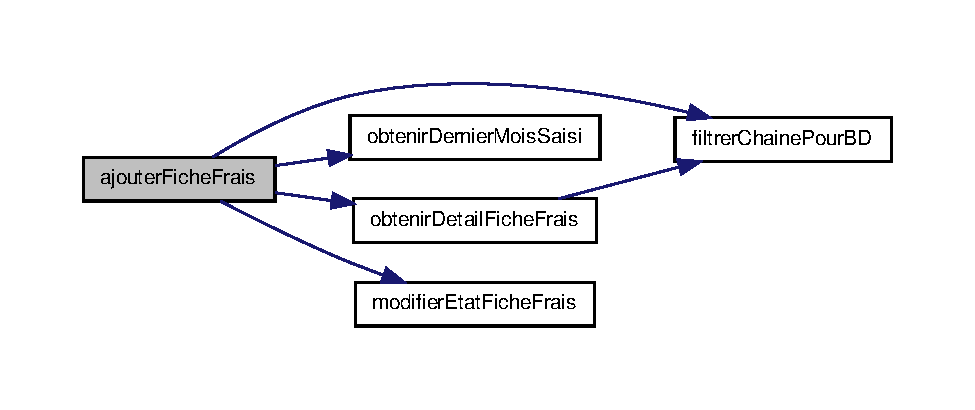
\includegraphics[width=350pt]{__bd_gestion_donnees_8lib_8php_a493124b80e53529be81247852b149f96_cgraph}
\end{center}
\end{figure}


\hypertarget{__bd_gestion_donnees_8lib_8php_a004b6774c7d5f590198b8ae4ad1ab424}{\index{\-\_\-bd\-Gestion\-Donnees.\-lib.\-php@{\-\_\-bd\-Gestion\-Donnees.\-lib.\-php}!ajouter\-Ligne\-H\-F@{ajouter\-Ligne\-H\-F}}
\index{ajouter\-Ligne\-H\-F@{ajouter\-Ligne\-H\-F}!_bdGestionDonnees.lib.php@{\-\_\-bd\-Gestion\-Donnees.\-lib.\-php}}
\subsubsection[{ajouter\-Ligne\-H\-F}]{\setlength{\rightskip}{0pt plus 5cm}ajouter\-Ligne\-H\-F (
\begin{DoxyParamCaption}
\item[{}]{\$id\-Cnx, }
\item[{}]{\$un\-Mois, }
\item[{}]{\$un\-Id\-Visiteur, }
\item[{}]{\$une\-Date\-H\-F, }
\item[{}]{\$un\-Libelle\-H\-F, }
\item[{}]{\$un\-Montant\-H\-F}
\end{DoxyParamCaption}
)}}\label{__bd_gestion_donnees_8lib_8php_a004b6774c7d5f590198b8ae4ad1ab424}
Ajoute une nouvelle ligne hors forfait. Insère dans la B\-D la ligne hors forfait de libellé \$un\-Libelle\-H\-F du montant \$un\-Montant\-H\-F ayant eu lieu à la date \$une\-Date\-H\-F pour la fiche de frais du mois \$un\-Mois du visiteur d'id \$un\-Id\-Visiteur 
\begin{DoxyParams}[1]{Paramètres}
resource & {\em \$id\-Cnx} & identifiant de connexion \\
\hline
string & {\em \$un\-Mois} & mois demandé (A\-A\-M\-M\-M\-M) \\
\hline
string & {\em \$un\-Id\-Visiteur} & id du visiteur \\
\hline
string & {\em \$une\-Date\-H\-F} & date du frais hors forfait \\
\hline
string & {\em \$un\-Libelle\-H\-F} & libellé du frais hors forfait \\
\hline
double & {\em \$un\-Montant\-H\-F} & montant du frais hors forfait \\
\hline
\end{DoxyParams}
\begin{DoxyReturn}{Renvoie}
void 
\end{DoxyReturn}


Définition à la ligne 278 du fichier \-\_\-bd\-Gestion\-Donnees.\-lib.\-php.



Voici le graphe d'appel pour cette fonction \-:\nopagebreak
\begin{figure}[H]
\begin{center}
\leavevmode
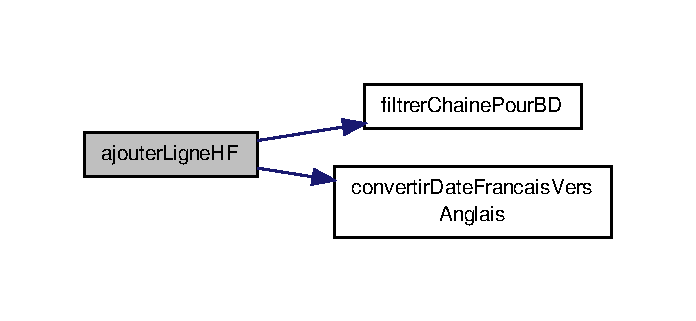
\includegraphics[width=334pt]{__bd_gestion_donnees_8lib_8php_a004b6774c7d5f590198b8ae4ad1ab424_cgraph}
\end{center}
\end{figure}


\hypertarget{__bd_gestion_donnees_8lib_8php_a3e03d598e990acf42577600cfe37f114}{\index{\-\_\-bd\-Gestion\-Donnees.\-lib.\-php@{\-\_\-bd\-Gestion\-Donnees.\-lib.\-php}!connecter\-Serveur\-B\-D@{connecter\-Serveur\-B\-D}}
\index{connecter\-Serveur\-B\-D@{connecter\-Serveur\-B\-D}!_bdGestionDonnees.lib.php@{\-\_\-bd\-Gestion\-Donnees.\-lib.\-php}}
\subsubsection[{connecter\-Serveur\-B\-D}]{\setlength{\rightskip}{0pt plus 5cm}connecter\-Serveur\-B\-D (
\begin{DoxyParamCaption}
{}
\end{DoxyParamCaption}
)}}\label{__bd_gestion_donnees_8lib_8php_a3e03d598e990acf42577600cfe37f114}
Se connecte au serveur de données My\-Sql. Se connecte au serveur de données My\-Sql à partir de valeurs prédéfinies de connexion (hôte, compte utilisateur et mot de passe). Retourne l'identifiant de connexion si succès obtenu, le booléen false si problème de connexion. \begin{DoxyReturn}{Renvoie}
resource identifiant de connexion 
\end{DoxyReturn}


Définition à la ligne 17 du fichier \-\_\-bd\-Gestion\-Donnees.\-lib.\-php.

\hypertarget{__bd_gestion_donnees_8lib_8php_aa443bd4a88ea69ec0e39ef82efd79f06}{\index{\-\_\-bd\-Gestion\-Donnees.\-lib.\-php@{\-\_\-bd\-Gestion\-Donnees.\-lib.\-php}!deconnecter\-Serveur\-B\-D@{deconnecter\-Serveur\-B\-D}}
\index{deconnecter\-Serveur\-B\-D@{deconnecter\-Serveur\-B\-D}!_bdGestionDonnees.lib.php@{\-\_\-bd\-Gestion\-Donnees.\-lib.\-php}}
\subsubsection[{deconnecter\-Serveur\-B\-D}]{\setlength{\rightskip}{0pt plus 5cm}deconnecter\-Serveur\-B\-D (
\begin{DoxyParamCaption}
\item[{}]{\$id\-Cnx}
\end{DoxyParamCaption}
)}}\label{__bd_gestion_donnees_8lib_8php_aa443bd4a88ea69ec0e39ef82efd79f06}
Ferme la connexion au serveur de données. Ferme la connexion au serveur de données identifiée par l'identifiant de connexion \$id\-Cnx. 
\begin{DoxyParams}[1]{Paramètres}
resource & {\em \$id\-Cnx} & identifiant de connexion \\
\hline
\end{DoxyParams}
\begin{DoxyReturn}{Renvoie}
void 
\end{DoxyReturn}


Définition à la ligne 47 du fichier \-\_\-bd\-Gestion\-Donnees.\-lib.\-php.

\hypertarget{__bd_gestion_donnees_8lib_8php_a0e6e5b420aed0486b7a9af7975739787}{\index{\-\_\-bd\-Gestion\-Donnees.\-lib.\-php@{\-\_\-bd\-Gestion\-Donnees.\-lib.\-php}!existe\-Fiche\-Frais@{existe\-Fiche\-Frais}}
\index{existe\-Fiche\-Frais@{existe\-Fiche\-Frais}!_bdGestionDonnees.lib.php@{\-\_\-bd\-Gestion\-Donnees.\-lib.\-php}}
\subsubsection[{existe\-Fiche\-Frais}]{\setlength{\rightskip}{0pt plus 5cm}existe\-Fiche\-Frais (
\begin{DoxyParamCaption}
\item[{}]{\$id\-Cnx, }
\item[{}]{\$un\-Mois, }
\item[{}]{\$un\-Id\-Visiteur}
\end{DoxyParamCaption}
)}}\label{__bd_gestion_donnees_8lib_8php_a0e6e5b420aed0486b7a9af7975739787}
Vérifie si une fiche de frais existe ou non. Retourne true si la fiche de frais du mois de \$un\-Mois (M\-M\-A\-A\-A\-A) du visiteur \$id\-Visiteur existe, false sinon. 
\begin{DoxyParams}[1]{Paramètres}
resource & {\em \$id\-Cnx} & identifiant de connexion \\
\hline
string & {\em \$un\-Mois} & mois demandé (M\-M\-A\-A\-A\-A) \\
\hline
string & {\em \$un\-Id\-Visiteur} & id visiteur \\
\hline
\end{DoxyParams}
\begin{DoxyReturn}{Renvoie}
booléen existence ou non de la fiche de frais 
\end{DoxyReturn}


Définition à la ligne 122 du fichier \-\_\-bd\-Gestion\-Donnees.\-lib.\-php.



Voici le graphe d'appel pour cette fonction \-:\nopagebreak
\begin{figure}[H]
\begin{center}
\leavevmode
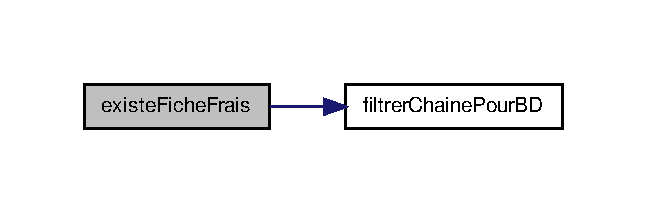
\includegraphics[width=310pt]{__bd_gestion_donnees_8lib_8php_a0e6e5b420aed0486b7a9af7975739787_cgraph}
\end{center}
\end{figure}


\hypertarget{__bd_gestion_donnees_8lib_8php_af2cca7a3ba7b15f9cedf99333367e598}{\index{\-\_\-bd\-Gestion\-Donnees.\-lib.\-php@{\-\_\-bd\-Gestion\-Donnees.\-lib.\-php}!filtrer\-Chaine\-Pour\-B\-D@{filtrer\-Chaine\-Pour\-B\-D}}
\index{filtrer\-Chaine\-Pour\-B\-D@{filtrer\-Chaine\-Pour\-B\-D}!_bdGestionDonnees.lib.php@{\-\_\-bd\-Gestion\-Donnees.\-lib.\-php}}
\subsubsection[{filtrer\-Chaine\-Pour\-B\-D}]{\setlength{\rightskip}{0pt plus 5cm}filtrer\-Chaine\-Pour\-B\-D (
\begin{DoxyParamCaption}
\item[{}]{\$str}
\end{DoxyParamCaption}
)}}\label{__bd_gestion_donnees_8lib_8php_af2cca7a3ba7b15f9cedf99333367e598}
Echappe les caractères spéciaux d'une chaîne. Envoie la chaîne \$str échappée, càd avec les caractères considérés spéciaux par My\-Sql (tq la quote simple) précédés d'un \textbackslash{}, ce qui annule leur effet spécial 
\begin{DoxyParams}[1]{Paramètres}
string & {\em \$str} & chaîne à échapper \\
\hline
\end{DoxyParams}
\begin{DoxyReturn}{Renvoie}
string chaîne échappée 
\end{DoxyReturn}


Définition à la ligne 58 du fichier \-\_\-bd\-Gestion\-Donnees.\-lib.\-php.



Voici le graphe des appelants de cette fonction \-:\nopagebreak
\begin{figure}[H]
\begin{center}
\leavevmode
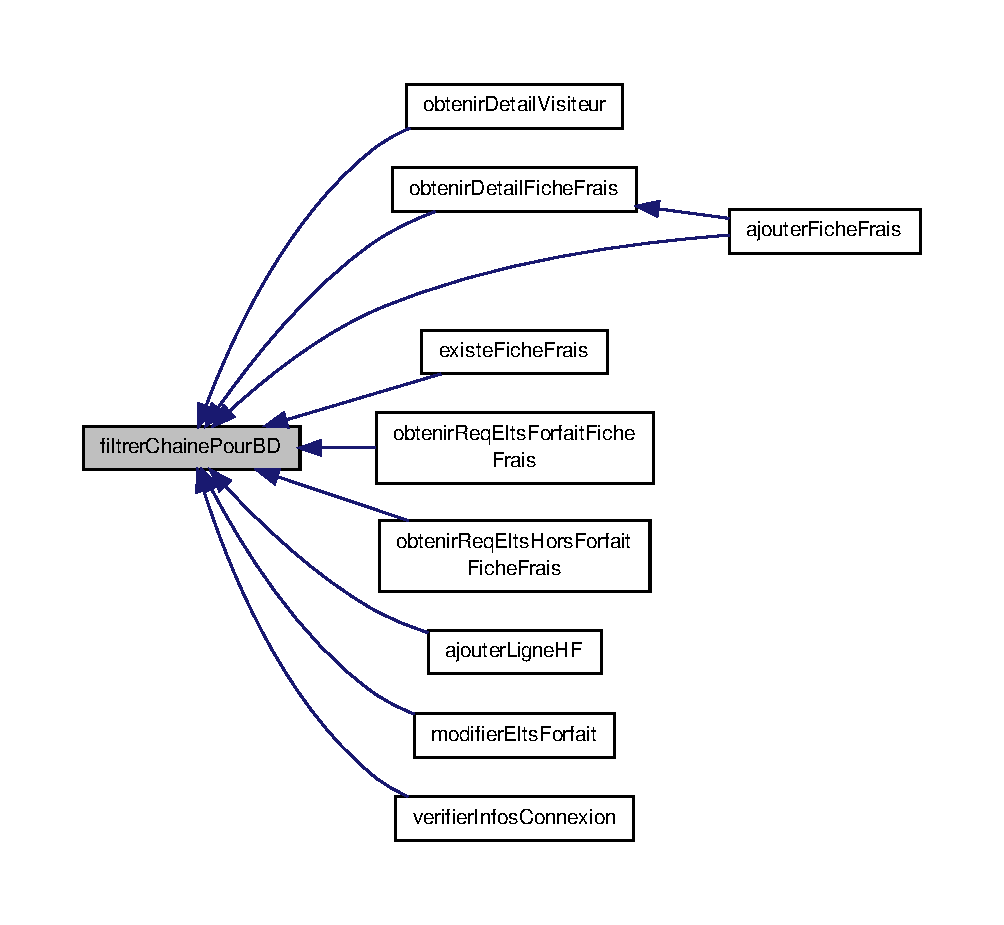
\includegraphics[width=350pt]{__bd_gestion_donnees_8lib_8php_af2cca7a3ba7b15f9cedf99333367e598_icgraph}
\end{center}
\end{figure}


\hypertarget{__bd_gestion_donnees_8lib_8php_a4471713bb3f5901d94f0e18de221e7a6}{\index{\-\_\-bd\-Gestion\-Donnees.\-lib.\-php@{\-\_\-bd\-Gestion\-Donnees.\-lib.\-php}!modifier\-Elts\-Forfait@{modifier\-Elts\-Forfait}}
\index{modifier\-Elts\-Forfait@{modifier\-Elts\-Forfait}!_bdGestionDonnees.lib.php@{\-\_\-bd\-Gestion\-Donnees.\-lib.\-php}}
\subsubsection[{modifier\-Elts\-Forfait}]{\setlength{\rightskip}{0pt plus 5cm}modifier\-Elts\-Forfait (
\begin{DoxyParamCaption}
\item[{}]{\$id\-Cnx, }
\item[{}]{\$un\-Mois, }
\item[{}]{\$un\-Id\-Visiteur, }
\item[{}]{\$des\-Elts\-Forfait}
\end{DoxyParamCaption}
)}}\label{__bd_gestion_donnees_8lib_8php_a4471713bb3f5901d94f0e18de221e7a6}
Modifie les quantités des éléments forfaitisés d'une fiche de frais. Met à jour les éléments forfaitisés contenus dans \$des\-Elts\-Forfaits pour le visiteur \$un\-Id\-Visiteur et le mois \$un\-Mois dans la table Ligne\-Frais\-Forfait, après avoir filtré (annulé l'effet de certains caractères considérés comme spéciaux par My\-Sql) chaque donnée 
\begin{DoxyParams}[1]{Paramètres}
resource & {\em \$id\-Cnx} & identifiant de connexion \\
\hline
string & {\em \$un\-Mois} & mois demandé (M\-M\-A\-A\-A\-A) \\
\hline
string & {\em \$un\-Id\-Visiteur} & id visiteur \\
\hline
array & {\em \$des\-Elts\-Forfait} & tableau des quantités des éléments hors forfait avec pour clés les identifiants des frais forfaitisés \\
\hline
\end{DoxyParams}
\begin{DoxyReturn}{Renvoie}
void 
\end{DoxyReturn}


Définition à la ligne 301 du fichier \-\_\-bd\-Gestion\-Donnees.\-lib.\-php.



Voici le graphe d'appel pour cette fonction \-:\nopagebreak
\begin{figure}[H]
\begin{center}
\leavevmode
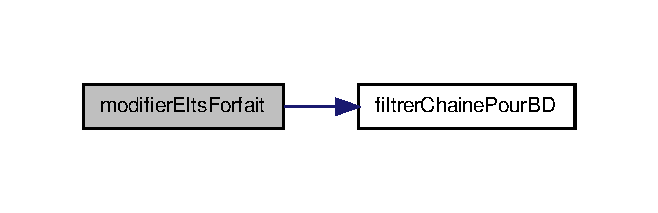
\includegraphics[width=316pt]{__bd_gestion_donnees_8lib_8php_a4471713bb3f5901d94f0e18de221e7a6_cgraph}
\end{center}
\end{figure}


\hypertarget{__bd_gestion_donnees_8lib_8php_a6f2b26d8059c5c5ad5967b976dd0915d}{\index{\-\_\-bd\-Gestion\-Donnees.\-lib.\-php@{\-\_\-bd\-Gestion\-Donnees.\-lib.\-php}!modifier\-Etat\-Fiche\-Frais@{modifier\-Etat\-Fiche\-Frais}}
\index{modifier\-Etat\-Fiche\-Frais@{modifier\-Etat\-Fiche\-Frais}!_bdGestionDonnees.lib.php@{\-\_\-bd\-Gestion\-Donnees.\-lib.\-php}}
\subsubsection[{modifier\-Etat\-Fiche\-Frais}]{\setlength{\rightskip}{0pt plus 5cm}modifier\-Etat\-Fiche\-Frais (
\begin{DoxyParamCaption}
\item[{}]{\$id\-Cnx, }
\item[{}]{\$un\-Mois, }
\item[{}]{\$un\-Id\-Visiteur, }
\item[{}]{\$un\-Etat}
\end{DoxyParamCaption}
)}}\label{__bd_gestion_donnees_8lib_8php_a6f2b26d8059c5c5ad5967b976dd0915d}
Modifie l'état et la date de modification d'une fiche de frais

Met à jour l'état de la fiche de frais du visiteur \$un\-Id\-Visiteur pour le mois \$un\-Mois à la nouvelle valeur \$un\-Etat et passe la date de modif à la date d'aujourd'hui 
\begin{DoxyParams}[1]{Paramètres}
resource & {\em \$id\-Cnx} & identifiant de connexion \\
\hline
string & {\em \$un\-Id\-Visiteur} & \\
\hline
string & {\em \$un\-Mois} & mois sous la forme aaaamm \\
\hline
\end{DoxyParams}
\begin{DoxyReturn}{Renvoie}
void 
\end{DoxyReturn}


Définition à la ligne 348 du fichier \-\_\-bd\-Gestion\-Donnees.\-lib.\-php.



Voici le graphe des appelants de cette fonction \-:\nopagebreak
\begin{figure}[H]
\begin{center}
\leavevmode
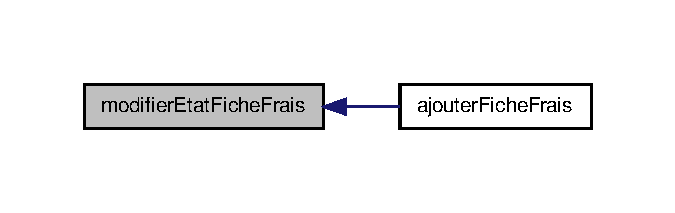
\includegraphics[width=324pt]{__bd_gestion_donnees_8lib_8php_a6f2b26d8059c5c5ad5967b976dd0915d_icgraph}
\end{center}
\end{figure}


\hypertarget{__bd_gestion_donnees_8lib_8php_a43c72282ff5396e3b67cc87753da4383}{\index{\-\_\-bd\-Gestion\-Donnees.\-lib.\-php@{\-\_\-bd\-Gestion\-Donnees.\-lib.\-php}!obtenir\-Dernier\-Mois\-Saisi@{obtenir\-Dernier\-Mois\-Saisi}}
\index{obtenir\-Dernier\-Mois\-Saisi@{obtenir\-Dernier\-Mois\-Saisi}!_bdGestionDonnees.lib.php@{\-\_\-bd\-Gestion\-Donnees.\-lib.\-php}}
\subsubsection[{obtenir\-Dernier\-Mois\-Saisi}]{\setlength{\rightskip}{0pt plus 5cm}obtenir\-Dernier\-Mois\-Saisi (
\begin{DoxyParamCaption}
\item[{}]{\$id\-Cnx, }
\item[{}]{\$un\-Id\-Visiteur}
\end{DoxyParamCaption}
)}}\label{__bd_gestion_donnees_8lib_8php_a43c72282ff5396e3b67cc87753da4383}
Fournit le mois de la dernière fiche de frais d'un visiteur. Retourne le mois de la dernière fiche de frais du visiteur d'id \$un\-Id\-Visiteur. 
\begin{DoxyParams}[1]{Paramètres}
resource & {\em \$id\-Cnx} & identifiant de connexion \\
\hline
string & {\em \$un\-Id\-Visiteur} & id visiteur \\
\hline
\end{DoxyParams}
\begin{DoxyReturn}{Renvoie}
string dernier mois sous la forme A\-A\-A\-A\-M\-M 
\end{DoxyReturn}


Définition à la ligne 144 du fichier \-\_\-bd\-Gestion\-Donnees.\-lib.\-php.



Voici le graphe des appelants de cette fonction \-:\nopagebreak
\begin{figure}[H]
\begin{center}
\leavevmode
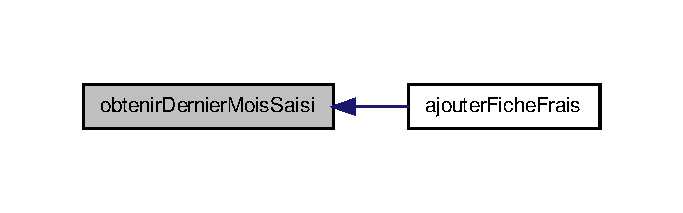
\includegraphics[width=328pt]{__bd_gestion_donnees_8lib_8php_a43c72282ff5396e3b67cc87753da4383_icgraph}
\end{center}
\end{figure}


\hypertarget{__bd_gestion_donnees_8lib_8php_a6119c74cdb5769c2a42bc14232cfc235}{\index{\-\_\-bd\-Gestion\-Donnees.\-lib.\-php@{\-\_\-bd\-Gestion\-Donnees.\-lib.\-php}!obtenir\-Detail\-Fiche\-Frais@{obtenir\-Detail\-Fiche\-Frais}}
\index{obtenir\-Detail\-Fiche\-Frais@{obtenir\-Detail\-Fiche\-Frais}!_bdGestionDonnees.lib.php@{\-\_\-bd\-Gestion\-Donnees.\-lib.\-php}}
\subsubsection[{obtenir\-Detail\-Fiche\-Frais}]{\setlength{\rightskip}{0pt plus 5cm}obtenir\-Detail\-Fiche\-Frais (
\begin{DoxyParamCaption}
\item[{}]{\$id\-Cnx, }
\item[{}]{\$un\-Mois, }
\item[{}]{\$un\-Id\-Visiteur}
\end{DoxyParamCaption}
)}}\label{__bd_gestion_donnees_8lib_8php_a6119c74cdb5769c2a42bc14232cfc235}
Fournit les informations d'une fiche de frais. Retourne les informations de la fiche de frais du mois de \$un\-Mois (M\-M\-A\-A\-A\-A) sous la forme d'un tableau associatif dont les clés sont les noms des colonnes (nb\-Justitificatifs, id\-Etat, libelle\-Etat, date\-Modif, montant\-Valide). 
\begin{DoxyParams}[1]{Paramètres}
resource & {\em \$id\-Cnx} & identifiant de connexion \\
\hline
string & {\em \$un\-Mois} & mois demandé (M\-M\-A\-A\-A\-A) \\
\hline
string & {\em \$un\-Id\-Visiteur} & id visiteur \\
\hline
\end{DoxyParams}
\begin{DoxyReturn}{Renvoie}
array tableau associatif de la fiche de frais 
\end{DoxyReturn}


Définition à la ligne 98 du fichier \-\_\-bd\-Gestion\-Donnees.\-lib.\-php.



Voici le graphe d'appel pour cette fonction \-:\nopagebreak
\begin{figure}[H]
\begin{center}
\leavevmode
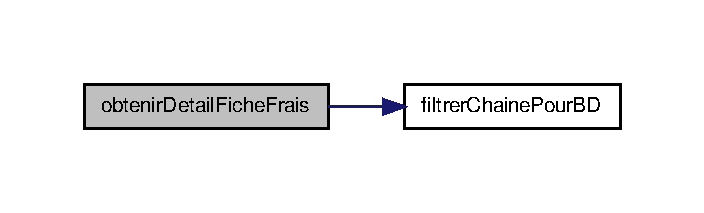
\includegraphics[width=338pt]{__bd_gestion_donnees_8lib_8php_a6119c74cdb5769c2a42bc14232cfc235_cgraph}
\end{center}
\end{figure}




Voici le graphe des appelants de cette fonction \-:\nopagebreak
\begin{figure}[H]
\begin{center}
\leavevmode
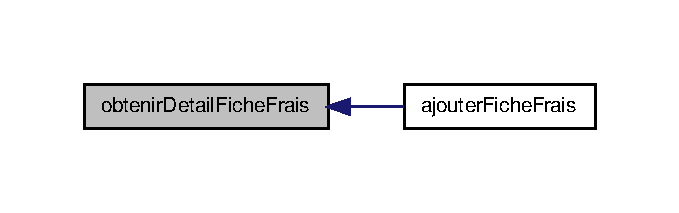
\includegraphics[width=326pt]{__bd_gestion_donnees_8lib_8php_a6119c74cdb5769c2a42bc14232cfc235_icgraph}
\end{center}
\end{figure}


\hypertarget{__bd_gestion_donnees_8lib_8php_a3d9b6723fcf62f7ccd5658e6b9485977}{\index{\-\_\-bd\-Gestion\-Donnees.\-lib.\-php@{\-\_\-bd\-Gestion\-Donnees.\-lib.\-php}!obtenir\-Detail\-Visiteur@{obtenir\-Detail\-Visiteur}}
\index{obtenir\-Detail\-Visiteur@{obtenir\-Detail\-Visiteur}!_bdGestionDonnees.lib.php@{\-\_\-bd\-Gestion\-Donnees.\-lib.\-php}}
\subsubsection[{obtenir\-Detail\-Visiteur}]{\setlength{\rightskip}{0pt plus 5cm}obtenir\-Detail\-Visiteur (
\begin{DoxyParamCaption}
\item[{}]{\$id\-Cnx, }
\item[{}]{\$un\-Id}
\end{DoxyParamCaption}
)}}\label{__bd_gestion_donnees_8lib_8php_a3d9b6723fcf62f7ccd5658e6b9485977}
Fournit les informations sur un visiteur demandé. Retourne les informations du visiteur d'id \$un\-Id sous la forme d'un tableau associatif dont les clés sont les noms des colonnes(id, nom, prenom). 
\begin{DoxyParams}[1]{Paramètres}
resource & {\em \$id\-Cnx} & identifiant de connexion \\
\hline
string & {\em \$un\-Id} & id de l'utilisateur \\
\hline
\end{DoxyParams}
\begin{DoxyReturn}{Renvoie}
array tableau associatif du visiteur 
\end{DoxyReturn}


Définition à la ligne 76 du fichier \-\_\-bd\-Gestion\-Donnees.\-lib.\-php.



Voici le graphe d'appel pour cette fonction \-:\nopagebreak
\begin{figure}[H]
\begin{center}
\leavevmode
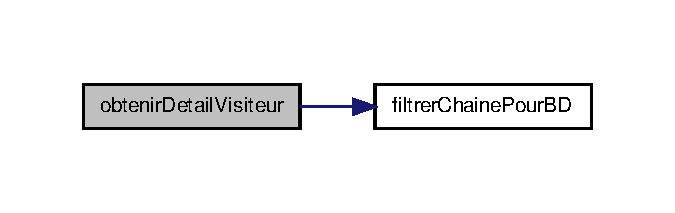
\includegraphics[width=324pt]{__bd_gestion_donnees_8lib_8php_a3d9b6723fcf62f7ccd5658e6b9485977_cgraph}
\end{center}
\end{figure}


\hypertarget{__bd_gestion_donnees_8lib_8php_a8a9e576b89da1f4174e8730e2a66873b}{\index{\-\_\-bd\-Gestion\-Donnees.\-lib.\-php@{\-\_\-bd\-Gestion\-Donnees.\-lib.\-php}!obtenir\-Req\-Elts\-Forfait\-Fiche\-Frais@{obtenir\-Req\-Elts\-Forfait\-Fiche\-Frais}}
\index{obtenir\-Req\-Elts\-Forfait\-Fiche\-Frais@{obtenir\-Req\-Elts\-Forfait\-Fiche\-Frais}!_bdGestionDonnees.lib.php@{\-\_\-bd\-Gestion\-Donnees.\-lib.\-php}}
\subsubsection[{obtenir\-Req\-Elts\-Forfait\-Fiche\-Frais}]{\setlength{\rightskip}{0pt plus 5cm}obtenir\-Req\-Elts\-Forfait\-Fiche\-Frais (
\begin{DoxyParamCaption}
\item[{}]{\$un\-Mois, }
\item[{}]{\$un\-Id\-Visiteur}
\end{DoxyParamCaption}
)}}\label{__bd_gestion_donnees_8lib_8php_a8a9e576b89da1f4174e8730e2a66873b}
Retourne le texte de la requète select concernant les éléments forfaitisés d'un visiteur pour un mois donnés.

La requète de sélection fournie permettra d'obtenir l'id, le libellé et la quantité des éléments forfaitisés de la fiche de frais du visiteur d'id \$id\-Visiteur pour le mois \$mois 
\begin{DoxyParams}[1]{Paramètres}
string & {\em \$un\-Mois} & mois demandé (M\-M\-A\-A\-A\-A) \\
\hline
string & {\em \$un\-Id\-Visiteur} & id visiteur \\
\hline
\end{DoxyParams}
\begin{DoxyReturn}{Renvoie}
string texte de la requète select 
\end{DoxyReturn}


Définition à la ligne 226 du fichier \-\_\-bd\-Gestion\-Donnees.\-lib.\-php.



Voici le graphe d'appel pour cette fonction \-:\nopagebreak
\begin{figure}[H]
\begin{center}
\leavevmode
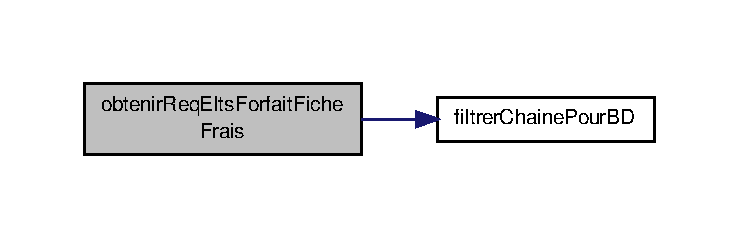
\includegraphics[width=350pt]{__bd_gestion_donnees_8lib_8php_a8a9e576b89da1f4174e8730e2a66873b_cgraph}
\end{center}
\end{figure}


\hypertarget{__bd_gestion_donnees_8lib_8php_a0c288b49f3dac1ab111e800f2794aac4}{\index{\-\_\-bd\-Gestion\-Donnees.\-lib.\-php@{\-\_\-bd\-Gestion\-Donnees.\-lib.\-php}!obtenir\-Req\-Elts\-Hors\-Forfait\-Fiche\-Frais@{obtenir\-Req\-Elts\-Hors\-Forfait\-Fiche\-Frais}}
\index{obtenir\-Req\-Elts\-Hors\-Forfait\-Fiche\-Frais@{obtenir\-Req\-Elts\-Hors\-Forfait\-Fiche\-Frais}!_bdGestionDonnees.lib.php@{\-\_\-bd\-Gestion\-Donnees.\-lib.\-php}}
\subsubsection[{obtenir\-Req\-Elts\-Hors\-Forfait\-Fiche\-Frais}]{\setlength{\rightskip}{0pt plus 5cm}obtenir\-Req\-Elts\-Hors\-Forfait\-Fiche\-Frais (
\begin{DoxyParamCaption}
\item[{}]{\$un\-Mois, }
\item[{}]{\$un\-Id\-Visiteur}
\end{DoxyParamCaption}
)}}\label{__bd_gestion_donnees_8lib_8php_a0c288b49f3dac1ab111e800f2794aac4}
Retourne le texte de la requète select concernant les éléments hors forfait d'un visiteur pour un mois donnés.

La requète de sélection fournie permettra d'obtenir l'id, la date, le libellé et le montant des éléments hors forfait de la fiche de frais du visiteur d'id \$id\-Visiteur pour le mois \$mois 
\begin{DoxyParams}[1]{Paramètres}
string & {\em \$un\-Mois} & mois demandé (M\-M\-A\-A\-A\-A) \\
\hline
string & {\em \$un\-Id\-Visiteur} & id visiteur \\
\hline
\end{DoxyParams}
\begin{DoxyReturn}{Renvoie}
string texte de la requète select 
\end{DoxyReturn}


Définition à la ligne 245 du fichier \-\_\-bd\-Gestion\-Donnees.\-lib.\-php.



Voici le graphe d'appel pour cette fonction \-:\nopagebreak
\begin{figure}[H]
\begin{center}
\leavevmode
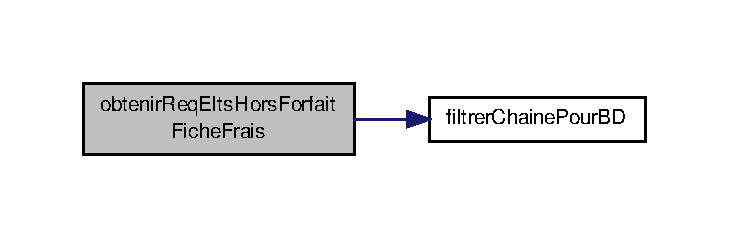
\includegraphics[width=350pt]{__bd_gestion_donnees_8lib_8php_a0c288b49f3dac1ab111e800f2794aac4_cgraph}
\end{center}
\end{figure}


\hypertarget{__bd_gestion_donnees_8lib_8php_af7ab441030c5c590de0b463414880a16}{\index{\-\_\-bd\-Gestion\-Donnees.\-lib.\-php@{\-\_\-bd\-Gestion\-Donnees.\-lib.\-php}!obtenir\-Req\-Mois\-Fiche\-Frais@{obtenir\-Req\-Mois\-Fiche\-Frais}}
\index{obtenir\-Req\-Mois\-Fiche\-Frais@{obtenir\-Req\-Mois\-Fiche\-Frais}!_bdGestionDonnees.lib.php@{\-\_\-bd\-Gestion\-Donnees.\-lib.\-php}}
\subsubsection[{obtenir\-Req\-Mois\-Fiche\-Frais}]{\setlength{\rightskip}{0pt plus 5cm}obtenir\-Req\-Mois\-Fiche\-Frais (
\begin{DoxyParamCaption}
\item[{}]{\$un\-Id\-Visiteur}
\end{DoxyParamCaption}
)}}\label{__bd_gestion_donnees_8lib_8php_af7ab441030c5c590de0b463414880a16}
Retourne le texte de la requète select concernant les mois pour lesquels un visiteur a une fiche de frais.

La requète de sélection fournie permettra d'obtenir les mois (A\-A\-A\-A\-M\-M) pour lesquels le visiteur \$un\-Id\-Visiteur a une fiche de frais. 
\begin{DoxyParams}[1]{Paramètres}
string & {\em \$un\-Id\-Visiteur} & id visiteur \\
\hline
\end{DoxyParams}
\begin{DoxyReturn}{Renvoie}
string texte de la requète select 
\end{DoxyReturn}


Définition à la ligne 209 du fichier \-\_\-bd\-Gestion\-Donnees.\-lib.\-php.

\hypertarget{__bd_gestion_donnees_8lib_8php_aa1a490dbef0da5c098e871f4091b910f}{\index{\-\_\-bd\-Gestion\-Donnees.\-lib.\-php@{\-\_\-bd\-Gestion\-Donnees.\-lib.\-php}!supprimer\-Ligne\-H\-F@{supprimer\-Ligne\-H\-F}}
\index{supprimer\-Ligne\-H\-F@{supprimer\-Ligne\-H\-F}!_bdGestionDonnees.lib.php@{\-\_\-bd\-Gestion\-Donnees.\-lib.\-php}}
\subsubsection[{supprimer\-Ligne\-H\-F}]{\setlength{\rightskip}{0pt plus 5cm}supprimer\-Ligne\-H\-F (
\begin{DoxyParamCaption}
\item[{}]{\$id\-Cnx, }
\item[{}]{\$un\-Id\-Ligne\-H\-F}
\end{DoxyParamCaption}
)}}\label{__bd_gestion_donnees_8lib_8php_aa1a490dbef0da5c098e871f4091b910f}
Supprime une ligne hors forfait. Supprime dans la B\-D la ligne hors forfait d'id \$un\-Id\-Ligne\-H\-F 
\begin{DoxyParams}[1]{Paramètres}
resource & {\em \$id\-Cnx} & identifiant de connexion \\
\hline
string & {\em \$id\-Ligne\-H\-F} & id de la ligne hors forfait \\
\hline
\end{DoxyParams}
\begin{DoxyReturn}{Renvoie}
void 
\end{DoxyReturn}


Définition à la ligne 260 du fichier \-\_\-bd\-Gestion\-Donnees.\-lib.\-php.

\hypertarget{__bd_gestion_donnees_8lib_8php_a67ac93fb32572194c13d3d2dca86af73}{\index{\-\_\-bd\-Gestion\-Donnees.\-lib.\-php@{\-\_\-bd\-Gestion\-Donnees.\-lib.\-php}!verifier\-Infos\-Connexion@{verifier\-Infos\-Connexion}}
\index{verifier\-Infos\-Connexion@{verifier\-Infos\-Connexion}!_bdGestionDonnees.lib.php@{\-\_\-bd\-Gestion\-Donnees.\-lib.\-php}}
\subsubsection[{verifier\-Infos\-Connexion}]{\setlength{\rightskip}{0pt plus 5cm}verifier\-Infos\-Connexion (
\begin{DoxyParamCaption}
\item[{}]{\$id\-Cnx, }
\item[{}]{\$un\-Login, }
\item[{}]{\$un\-Mdp}
\end{DoxyParamCaption}
)}}\label{__bd_gestion_donnees_8lib_8php_a67ac93fb32572194c13d3d2dca86af73}
Contrôle les informations de connexionn d'un utilisateur. Vérifie si les informations de connexion \$un\-Login, \$un\-Mdp sont ou non valides. Retourne les informations de l'utilisateur sous forme de tableau associatif dont les clés sont les noms des colonnes (id, nom, prenom, login, mdp) si login et mot de passe existent, le booléen false sinon. 
\begin{DoxyParams}[1]{Paramètres}
resource & {\em \$id\-Cnx} & identifiant de connexion \\
\hline
string & {\em \$un\-Login} & login \\
\hline
string & {\em \$un\-Mdp} & mot de passe \\
\hline
\end{DoxyParams}
\begin{DoxyReturn}{Renvoie}
array tableau associatif ou booléen false 
\end{DoxyReturn}


Définition à la ligne 323 du fichier \-\_\-bd\-Gestion\-Donnees.\-lib.\-php.



Voici le graphe d'appel pour cette fonction \-:\nopagebreak
\begin{figure}[H]
\begin{center}
\leavevmode
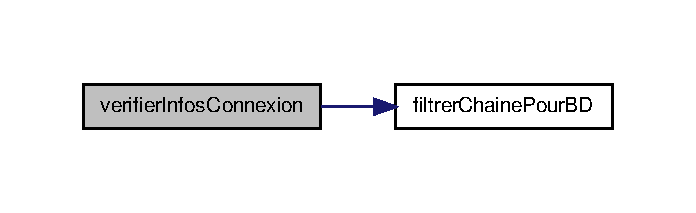
\includegraphics[width=334pt]{__bd_gestion_donnees_8lib_8php_a67ac93fb32572194c13d3d2dca86af73_cgraph}
\end{center}
\end{figure}



\hypertarget{__fin_8inc_8php}{\section{Référence du fichier /home/trackoen/\-P\-H\-P\-\_\-\-P\-R\-O\-J\-E\-C\-T/\-G\-S\-B\-\_\-\-Appli/include/\-\_\-fin.inc.\-php}
\label{__fin_8inc_8php}\index{/home/trackoen/\-P\-H\-P\-\_\-\-P\-R\-O\-J\-E\-C\-T/\-G\-S\-B\-\_\-\-Appli/include/\-\_\-fin.\-inc.\-php@{/home/trackoen/\-P\-H\-P\-\_\-\-P\-R\-O\-J\-E\-C\-T/\-G\-S\-B\-\_\-\-Appli/include/\-\_\-fin.\-inc.\-php}}
}
\subsection*{Espaces de nommage}
\begin{DoxyCompactItemize}
\item 
namespace \hyperlink{namespacedefault}{default}
\end{DoxyCompactItemize}

\hypertarget{__gestion_session_8lib_8php}{\section{Référence du fichier /home/trackoen/\-P\-H\-P\-\_\-\-P\-R\-O\-J\-E\-C\-T/\-G\-S\-B\-\_\-\-Appli/include/\-\_\-gestion\-Session.lib.\-php}
\label{__gestion_session_8lib_8php}\index{/home/trackoen/\-P\-H\-P\-\_\-\-P\-R\-O\-J\-E\-C\-T/\-G\-S\-B\-\_\-\-Appli/include/\-\_\-gestion\-Session.\-lib.\-php@{/home/trackoen/\-P\-H\-P\-\_\-\-P\-R\-O\-J\-E\-C\-T/\-G\-S\-B\-\_\-\-Appli/include/\-\_\-gestion\-Session.\-lib.\-php}}
}
\subsection*{Espaces de nommage}
\begin{DoxyCompactItemize}
\item 
namespace \hyperlink{namespacedefault}{default}
\end{DoxyCompactItemize}
\subsection*{Fonctions}
\begin{DoxyCompactItemize}
\item 
\hyperlink{__gestion_session_8lib_8php_a59570c6f011b3618075794d8ae341d50}{init\-Session} ()
\item 
\hyperlink{__gestion_session_8lib_8php_a7af627b049f30bda0af2678c3327aff0}{obtenir\-Id\-User\-Connecte} ()
\item 
\hyperlink{__gestion_session_8lib_8php_a6e2d96c04d04362c4b3e84abe3d79640}{affecter\-Infos\-Connecte} (\$id, \$login)
\item 
\hyperlink{__gestion_session_8lib_8php_ae31f1b8a9f65a7180483f4d79c478a6e}{deconnecter\-Visiteur} ()
\item 
\hyperlink{__gestion_session_8lib_8php_afe911e51f16958708b8b700981cd2567}{est\-Visiteur\-Connecte} ()
\end{DoxyCompactItemize}


\subsection{Documentation des fonctions}
\hypertarget{__gestion_session_8lib_8php_a6e2d96c04d04362c4b3e84abe3d79640}{\index{\-\_\-gestion\-Session.\-lib.\-php@{\-\_\-gestion\-Session.\-lib.\-php}!affecter\-Infos\-Connecte@{affecter\-Infos\-Connecte}}
\index{affecter\-Infos\-Connecte@{affecter\-Infos\-Connecte}!_gestionSession.lib.php@{\-\_\-gestion\-Session.\-lib.\-php}}
\subsubsection[{affecter\-Infos\-Connecte}]{\setlength{\rightskip}{0pt plus 5cm}affecter\-Infos\-Connecte (
\begin{DoxyParamCaption}
\item[{}]{\$id, }
\item[{}]{\$login}
\end{DoxyParamCaption}
)}}\label{__gestion_session_8lib_8php_a6e2d96c04d04362c4b3e84abe3d79640}
Conserve en variables session les informations du visiteur connecté

Conserve en variables session l'id \$id et le login \$login du visiteur connecté 
\begin{DoxyParams}{Paramètres}
{\em string} & id du visiteur \\
\hline
{\em string} & login du visiteur \\
\hline
\end{DoxyParams}
\begin{DoxyReturn}{Renvoie}
void 
\end{DoxyReturn}


Définition à la ligne 39 du fichier \-\_\-gestion\-Session.\-lib.\-php.

\hypertarget{__gestion_session_8lib_8php_ae31f1b8a9f65a7180483f4d79c478a6e}{\index{\-\_\-gestion\-Session.\-lib.\-php@{\-\_\-gestion\-Session.\-lib.\-php}!deconnecter\-Visiteur@{deconnecter\-Visiteur}}
\index{deconnecter\-Visiteur@{deconnecter\-Visiteur}!_gestionSession.lib.php@{\-\_\-gestion\-Session.\-lib.\-php}}
\subsubsection[{deconnecter\-Visiteur}]{\setlength{\rightskip}{0pt plus 5cm}deconnecter\-Visiteur (
\begin{DoxyParamCaption}
{}
\end{DoxyParamCaption}
)}}\label{__gestion_session_8lib_8php_ae31f1b8a9f65a7180483f4d79c478a6e}
Déconnecte le visiteur qui s'est identifié sur le site.

\begin{DoxyReturn}{Renvoie}
void 
\end{DoxyReturn}


Définition à la ligne 49 du fichier \-\_\-gestion\-Session.\-lib.\-php.

\hypertarget{__gestion_session_8lib_8php_afe911e51f16958708b8b700981cd2567}{\index{\-\_\-gestion\-Session.\-lib.\-php@{\-\_\-gestion\-Session.\-lib.\-php}!est\-Visiteur\-Connecte@{est\-Visiteur\-Connecte}}
\index{est\-Visiteur\-Connecte@{est\-Visiteur\-Connecte}!_gestionSession.lib.php@{\-\_\-gestion\-Session.\-lib.\-php}}
\subsubsection[{est\-Visiteur\-Connecte}]{\setlength{\rightskip}{0pt plus 5cm}est\-Visiteur\-Connecte (
\begin{DoxyParamCaption}
{}
\end{DoxyParamCaption}
)}}\label{__gestion_session_8lib_8php_afe911e51f16958708b8b700981cd2567}
Vérifie si un visiteur s'est connecté sur le site.

Retourne true si un visiteur s'est identifié sur le site, false sinon. \begin{DoxyReturn}{Renvoie}
boolean échec ou succès 
\end{DoxyReturn}


Définition à la ligne 60 du fichier \-\_\-gestion\-Session.\-lib.\-php.

\hypertarget{__gestion_session_8lib_8php_a59570c6f011b3618075794d8ae341d50}{\index{\-\_\-gestion\-Session.\-lib.\-php@{\-\_\-gestion\-Session.\-lib.\-php}!init\-Session@{init\-Session}}
\index{init\-Session@{init\-Session}!_gestionSession.lib.php@{\-\_\-gestion\-Session.\-lib.\-php}}
\subsubsection[{init\-Session}]{\setlength{\rightskip}{0pt plus 5cm}init\-Session (
\begin{DoxyParamCaption}
{}
\end{DoxyParamCaption}
)}}\label{__gestion_session_8lib_8php_a59570c6f011b3618075794d8ae341d50}
Démarre ou poursuit une session.

\begin{DoxyReturn}{Renvoie}
void 
\end{DoxyReturn}


Définition à la ligne 13 du fichier \-\_\-gestion\-Session.\-lib.\-php.

\hypertarget{__gestion_session_8lib_8php_a7af627b049f30bda0af2678c3327aff0}{\index{\-\_\-gestion\-Session.\-lib.\-php@{\-\_\-gestion\-Session.\-lib.\-php}!obtenir\-Id\-User\-Connecte@{obtenir\-Id\-User\-Connecte}}
\index{obtenir\-Id\-User\-Connecte@{obtenir\-Id\-User\-Connecte}!_gestionSession.lib.php@{\-\_\-gestion\-Session.\-lib.\-php}}
\subsubsection[{obtenir\-Id\-User\-Connecte}]{\setlength{\rightskip}{0pt plus 5cm}obtenir\-Id\-User\-Connecte (
\begin{DoxyParamCaption}
{}
\end{DoxyParamCaption}
)}}\label{__gestion_session_8lib_8php_a7af627b049f30bda0af2678c3327aff0}
Fournit l'id du visiteur connecté.

Retourne l'id du visiteur connecté, une chaîne vide si pas de visiteur connecté. \begin{DoxyReturn}{Renvoie}
string id du visiteur connecté 
\end{DoxyReturn}


Définition à la ligne 23 du fichier \-\_\-gestion\-Session.\-lib.\-php.


\hypertarget{__init_8inc_8php}{\section{Référence du fichier /home/trackoen/\-P\-H\-P\-\_\-\-P\-R\-O\-J\-E\-C\-T/\-G\-S\-B\-\_\-\-Appli/include/\-\_\-init.inc.\-php}
\label{__init_8inc_8php}\index{/home/trackoen/\-P\-H\-P\-\_\-\-P\-R\-O\-J\-E\-C\-T/\-G\-S\-B\-\_\-\-Appli/include/\-\_\-init.\-inc.\-php@{/home/trackoen/\-P\-H\-P\-\_\-\-P\-R\-O\-J\-E\-C\-T/\-G\-S\-B\-\_\-\-Appli/include/\-\_\-init.\-inc.\-php}}
}
\subsection*{Espaces de nommage}
\begin{DoxyCompactItemize}
\item 
namespace \hyperlink{namespacedefault}{default}
\end{DoxyCompactItemize}
\subsection*{Variables}
\begin{DoxyCompactItemize}
\item 
\hyperlink{__init_8inc_8php_aaab0cf947dbef94de72bc55c49555684}{\$tab\-Erreurs} = array()
\item 
\hyperlink{__init_8inc_8php_a66aed633c4b3dc9690db4076a0a7edf5}{\$demande\-Deconnexion} = \hyperlink{__utilitaires_et_gestion_erreurs_8lib_8php_ad3618b973b51810a2eb97a0493ade9ee}{lire\-Donnee\-Url}(\char`\"{}cmd\-Deconnecter\char`\"{})
\item 
\hyperlink{c_se_connecter_8php_a161e098d41499c163a94c3fa5cd0e698}{if}(\$demande\-Deconnexion==\char`\"{}on\char`\"{}) \hyperlink{__init_8inc_8php_ae48ae6a6b06018043563b88782bd2bee}{\$id\-Connexion} = \hyperlink{__bd_gestion_donnees_8lib_8php_a3e03d598e990acf42577600cfe37f114}{connecter\-Serveur\-B\-D}()
\end{DoxyCompactItemize}


\subsection{Documentation des variables}
\hypertarget{__init_8inc_8php_a66aed633c4b3dc9690db4076a0a7edf5}{\index{\-\_\-init.\-inc.\-php@{\-\_\-init.\-inc.\-php}!\$demande\-Deconnexion@{\$demande\-Deconnexion}}
\index{\$demande\-Deconnexion@{\$demande\-Deconnexion}!_init.inc.php@{\-\_\-init.\-inc.\-php}}
\subsubsection[{\$demande\-Deconnexion}]{\setlength{\rightskip}{0pt plus 5cm}\$demande\-Deconnexion = {\bf lire\-Donnee\-Url}(\char`\"{}cmd\-Deconnecter\char`\"{})}}\label{__init_8inc_8php_a66aed633c4b3dc9690db4076a0a7edf5}


Définition à la ligne 16 du fichier \-\_\-init.\-inc.\-php.

\hypertarget{__init_8inc_8php_ae48ae6a6b06018043563b88782bd2bee}{\index{\-\_\-init.\-inc.\-php@{\-\_\-init.\-inc.\-php}!\$id\-Connexion@{\$id\-Connexion}}
\index{\$id\-Connexion@{\$id\-Connexion}!_init.inc.php@{\-\_\-init.\-inc.\-php}}
\subsubsection[{\$id\-Connexion}]{\setlength{\rightskip}{0pt plus 5cm}{\bf if} (\$demande\-Deconnexion==\char`\"{}on\char`\"{}) \$id\-Connexion = {\bf connecter\-Serveur\-B\-D}()}}\label{__init_8inc_8php_ae48ae6a6b06018043563b88782bd2bee}


Définition à la ligne 24 du fichier \-\_\-init.\-inc.\-php.

\hypertarget{__init_8inc_8php_aaab0cf947dbef94de72bc55c49555684}{\index{\-\_\-init.\-inc.\-php@{\-\_\-init.\-inc.\-php}!\$tab\-Erreurs@{\$tab\-Erreurs}}
\index{\$tab\-Erreurs@{\$tab\-Erreurs}!_init.inc.php@{\-\_\-init.\-inc.\-php}}
\subsubsection[{\$tab\-Erreurs}]{\setlength{\rightskip}{0pt plus 5cm}\$tab\-Erreurs = array()}}\label{__init_8inc_8php_aaab0cf947dbef94de72bc55c49555684}


Définition à la ligne 13 du fichier \-\_\-init.\-inc.\-php.


\hypertarget{__sommaire_8inc_8php}{\section{Référence du fichier /home/trackoen/\-P\-H\-P\-\_\-\-P\-R\-O\-J\-E\-C\-T/\-G\-S\-B\-\_\-\-Appli/include/\-\_\-sommaire.inc.\-php}
\label{__sommaire_8inc_8php}\index{/home/trackoen/\-P\-H\-P\-\_\-\-P\-R\-O\-J\-E\-C\-T/\-G\-S\-B\-\_\-\-Appli/include/\-\_\-sommaire.\-inc.\-php@{/home/trackoen/\-P\-H\-P\-\_\-\-P\-R\-O\-J\-E\-C\-T/\-G\-S\-B\-\_\-\-Appli/include/\-\_\-sommaire.\-inc.\-php}}
}

\hypertarget{__utilitaires_et_gestion_erreurs_8lib_8php}{\section{Référence du fichier /home/trackoen/\-P\-H\-P\-\_\-\-P\-R\-O\-J\-E\-C\-T/\-G\-S\-B\-\_\-\-Appli/include/\-\_\-utilitaires\-Et\-Gestion\-Erreurs.lib.\-php}
\label{__utilitaires_et_gestion_erreurs_8lib_8php}\index{/home/trackoen/\-P\-H\-P\-\_\-\-P\-R\-O\-J\-E\-C\-T/\-G\-S\-B\-\_\-\-Appli/include/\-\_\-utilitaires\-Et\-Gestion\-Erreurs.\-lib.\-php@{/home/trackoen/\-P\-H\-P\-\_\-\-P\-R\-O\-J\-E\-C\-T/\-G\-S\-B\-\_\-\-Appli/include/\-\_\-utilitaires\-Et\-Gestion\-Erreurs.\-lib.\-php}}
}
\subsection*{Espaces de nommage}
\begin{DoxyCompactItemize}
\item 
namespace \hyperlink{namespacedefault}{default}
\end{DoxyCompactItemize}
\subsection*{Fonctions}
\begin{DoxyCompactItemize}
\item 
\hyperlink{__utilitaires_et_gestion_erreurs_8lib_8php_a991bef919e2c370187e9d7eec29f8f50}{obtenir\-Libelle\-Mois} (\$un\-No\-Mois)
\item 
\hyperlink{__utilitaires_et_gestion_erreurs_8lib_8php_a4f7821728a7b40482111da18fc60603f}{est\-Date} (\$date)
\item 
\hyperlink{__utilitaires_et_gestion_erreurs_8lib_8php_a39cb4860d4761f8107a63bac07db4102}{convertir\-Date\-Francais\-Vers\-Anglais} (\$date)
\item 
\hyperlink{__utilitaires_et_gestion_erreurs_8lib_8php_ace9e1c93b7ce32b3ab1aa8f86e033e78}{convertir\-Date\-Anglais\-Vers\-Francais} (\$date)
\item 
\hyperlink{__utilitaires_et_gestion_erreurs_8lib_8php_a092454f070d08318790e482128089483}{est\-Dans\-Annee\-Ecoulee} (\$date)
\item 
\hyperlink{__utilitaires_et_gestion_erreurs_8lib_8php_a5891ac42bd25b5bb5a9427174f8eb15f}{est\-Entier\-Positif} (\$valeur)
\item 
\hyperlink{__utilitaires_et_gestion_erreurs_8lib_8php_a3457b44782886f81a118ee6ae62f9568}{verifier\-Entiers\-Positifs} (\$les\-Valeurs)
\item 
\hyperlink{__utilitaires_et_gestion_erreurs_8lib_8php_ad3618b973b51810a2eb97a0493ade9ee}{lire\-Donnee\-Url} (\$nom\-Donnee, \$val\-Defaut=\char`\"{}\char`\"{})
\item 
\hyperlink{__utilitaires_et_gestion_erreurs_8lib_8php_ab0070fc1ef4283caa3457dd5b71a86de}{lire\-Donnee\-Post} (\$nom\-Donnee, \$val\-Defaut=\char`\"{}\char`\"{})
\item 
\hyperlink{__utilitaires_et_gestion_erreurs_8lib_8php_ab4e61487d300e37e058c1fd31c0446a9}{lire\-Donnee} (\$nom\-Donnee, \$val\-Defaut=\char`\"{}\char`\"{})
\item 
\hyperlink{__utilitaires_et_gestion_erreurs_8lib_8php_a6958994232c9af063f867d133a044ab5}{ajouter\-Erreur} (\&\$tab\-Err, \$msg)
\item 
\hyperlink{__utilitaires_et_gestion_erreurs_8lib_8php_a61c228522012792b81b2931ef1ae32ce}{nb\-Erreurs} (\$tab\-Err)
\item 
\hyperlink{__utilitaires_et_gestion_erreurs_8lib_8php_a2ff214e84108237a421875ab1ab3f7fa}{to\-String\-Erreurs} (\$tab\-Err)
\item 
\hyperlink{__utilitaires_et_gestion_erreurs_8lib_8php_ad19609774a0abdc797f46e59df5aa55f}{filtrer\-Chaine\-Pour\-Navig} (\$str)
\item 
\hyperlink{__utilitaires_et_gestion_erreurs_8lib_8php_add1850973a586302c7fab9e20bd1dd25}{verifier\-Ligne\-Frais\-H\-F} (\$date, \$libelle, \$montant, \&\$tab\-Errs)
\end{DoxyCompactItemize}


\subsection{Documentation des fonctions}
\hypertarget{__utilitaires_et_gestion_erreurs_8lib_8php_a6958994232c9af063f867d133a044ab5}{\index{\-\_\-utilitaires\-Et\-Gestion\-Erreurs.\-lib.\-php@{\-\_\-utilitaires\-Et\-Gestion\-Erreurs.\-lib.\-php}!ajouter\-Erreur@{ajouter\-Erreur}}
\index{ajouter\-Erreur@{ajouter\-Erreur}!_utilitairesEtGestionErreurs.lib.php@{\-\_\-utilitaires\-Et\-Gestion\-Erreurs.\-lib.\-php}}
\subsubsection[{ajouter\-Erreur}]{\setlength{\rightskip}{0pt plus 5cm}ajouter\-Erreur (
\begin{DoxyParamCaption}
\item[{\&}]{\$tab\-Err, }
\item[{}]{\$msg}
\end{DoxyParamCaption}
)}}\label{__utilitaires_et_gestion_erreurs_8lib_8php_a6958994232c9af063f867d133a044ab5}
Ajoute un message dans le tableau des messages d'erreurs.

Ajoute le message \$msg en fin de tableau \$tab\-Err. Ce tableau est passé par référence afin que les modifications sur ce tableau soient visibles de l'appelant. 
\begin{DoxyParams}[1]{Paramètres}
array & {\em \$tab\-Err} & \\
\hline
 & {\em string} & message \\
\hline
\end{DoxyParams}
\begin{DoxyReturn}{Renvoie}
void 
\end{DoxyReturn}


Définition à la ligne 191 du fichier \-\_\-utilitaires\-Et\-Gestion\-Erreurs.\-lib.\-php.



Voici le graphe des appelants de cette fonction \-:\nopagebreak
\begin{figure}[H]
\begin{center}
\leavevmode
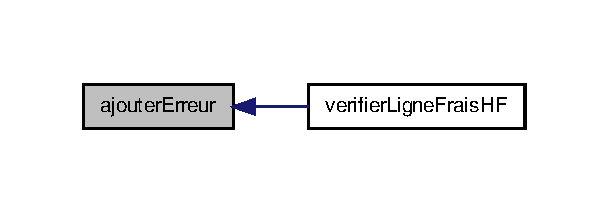
\includegraphics[width=292pt]{__utilitaires_et_gestion_erreurs_8lib_8php_a6958994232c9af063f867d133a044ab5_icgraph}
\end{center}
\end{figure}


\hypertarget{__utilitaires_et_gestion_erreurs_8lib_8php_ace9e1c93b7ce32b3ab1aa8f86e033e78}{\index{\-\_\-utilitaires\-Et\-Gestion\-Erreurs.\-lib.\-php@{\-\_\-utilitaires\-Et\-Gestion\-Erreurs.\-lib.\-php}!convertir\-Date\-Anglais\-Vers\-Francais@{convertir\-Date\-Anglais\-Vers\-Francais}}
\index{convertir\-Date\-Anglais\-Vers\-Francais@{convertir\-Date\-Anglais\-Vers\-Francais}!_utilitairesEtGestionErreurs.lib.php@{\-\_\-utilitaires\-Et\-Gestion\-Erreurs.\-lib.\-php}}
\subsubsection[{convertir\-Date\-Anglais\-Vers\-Francais}]{\setlength{\rightskip}{0pt plus 5cm}convertir\-Date\-Anglais\-Vers\-Francais (
\begin{DoxyParamCaption}
\item[{}]{\$date}
\end{DoxyParamCaption}
)}}\label{__utilitaires_et_gestion_erreurs_8lib_8php_ace9e1c93b7ce32b3ab1aa8f86e033e78}
Transforme une date au format format anglais aaaa-\/mm-\/jj vers le format français jj/mm/aaaa 
\begin{DoxyParams}{Paramètres}
{\em \$date} & au format aaaa-\/mm-\/jj \\
\hline
\end{DoxyParams}
\begin{DoxyReturn}{Renvoie}
string la date au format format français jj/mm/aaaa 
\end{DoxyReturn}


Définition à la ligne 67 du fichier \-\_\-utilitaires\-Et\-Gestion\-Erreurs.\-lib.\-php.

\hypertarget{__utilitaires_et_gestion_erreurs_8lib_8php_a39cb4860d4761f8107a63bac07db4102}{\index{\-\_\-utilitaires\-Et\-Gestion\-Erreurs.\-lib.\-php@{\-\_\-utilitaires\-Et\-Gestion\-Erreurs.\-lib.\-php}!convertir\-Date\-Francais\-Vers\-Anglais@{convertir\-Date\-Francais\-Vers\-Anglais}}
\index{convertir\-Date\-Francais\-Vers\-Anglais@{convertir\-Date\-Francais\-Vers\-Anglais}!_utilitairesEtGestionErreurs.lib.php@{\-\_\-utilitaires\-Et\-Gestion\-Erreurs.\-lib.\-php}}
\subsubsection[{convertir\-Date\-Francais\-Vers\-Anglais}]{\setlength{\rightskip}{0pt plus 5cm}convertir\-Date\-Francais\-Vers\-Anglais (
\begin{DoxyParamCaption}
\item[{}]{\$date}
\end{DoxyParamCaption}
)}}\label{__utilitaires_et_gestion_erreurs_8lib_8php_a39cb4860d4761f8107a63bac07db4102}
Transforme une date au format français jj/mm/aaaa vers le format anglais aaaa-\/mm-\/jj 
\begin{DoxyParams}{Paramètres}
{\em \$date} & au format jj/mm/aaaa \\
\hline
\end{DoxyParams}
\begin{DoxyReturn}{Renvoie}
string la date au format anglais aaaa-\/mm-\/jj 
\end{DoxyReturn}


Définition à la ligne 56 du fichier \-\_\-utilitaires\-Et\-Gestion\-Erreurs.\-lib.\-php.



Voici le graphe des appelants de cette fonction \-:\nopagebreak
\begin{figure}[H]
\begin{center}
\leavevmode
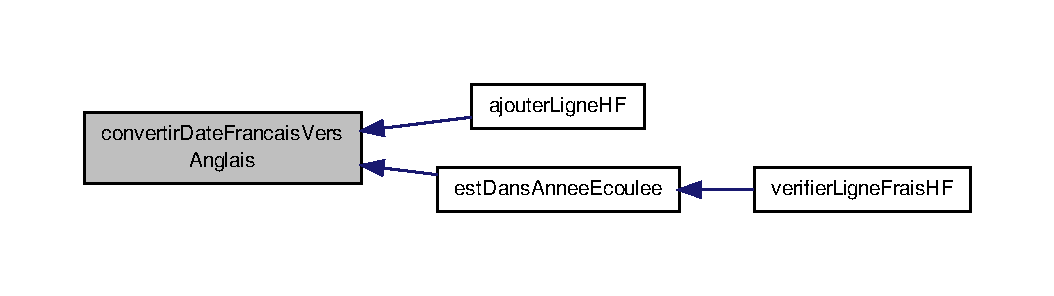
\includegraphics[width=350pt]{__utilitaires_et_gestion_erreurs_8lib_8php_a39cb4860d4761f8107a63bac07db4102_icgraph}
\end{center}
\end{figure}


\hypertarget{__utilitaires_et_gestion_erreurs_8lib_8php_a092454f070d08318790e482128089483}{\index{\-\_\-utilitaires\-Et\-Gestion\-Erreurs.\-lib.\-php@{\-\_\-utilitaires\-Et\-Gestion\-Erreurs.\-lib.\-php}!est\-Dans\-Annee\-Ecoulee@{est\-Dans\-Annee\-Ecoulee}}
\index{est\-Dans\-Annee\-Ecoulee@{est\-Dans\-Annee\-Ecoulee}!_utilitairesEtGestionErreurs.lib.php@{\-\_\-utilitaires\-Et\-Gestion\-Erreurs.\-lib.\-php}}
\subsubsection[{est\-Dans\-Annee\-Ecoulee}]{\setlength{\rightskip}{0pt plus 5cm}est\-Dans\-Annee\-Ecoulee (
\begin{DoxyParamCaption}
\item[{}]{\$date}
\end{DoxyParamCaption}
)}}\label{__utilitaires_et_gestion_erreurs_8lib_8php_a092454f070d08318790e482128089483}
Indique si une date est incluse ou non dans l'année écoulée.

Retourne true si la date \$date est comprise entre la date du jour moins un an et la la date du jour. False sinon. 
\begin{DoxyParams}{Paramètres}
{\em \$date} & date au format jj/mm/aaaa \\
\hline
\end{DoxyParams}
\begin{DoxyReturn}{Renvoie}
boolean succès ou échec 
\end{DoxyReturn}


Définition à la ligne 80 du fichier \-\_\-utilitaires\-Et\-Gestion\-Erreurs.\-lib.\-php.



Voici le graphe d'appel pour cette fonction \-:\nopagebreak
\begin{figure}[H]
\begin{center}
\leavevmode
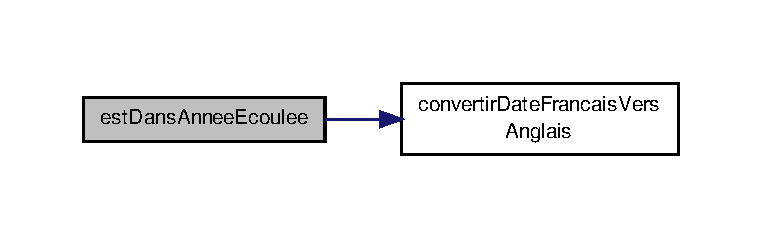
\includegraphics[width=350pt]{__utilitaires_et_gestion_erreurs_8lib_8php_a092454f070d08318790e482128089483_cgraph}
\end{center}
\end{figure}




Voici le graphe des appelants de cette fonction \-:\nopagebreak
\begin{figure}[H]
\begin{center}
\leavevmode
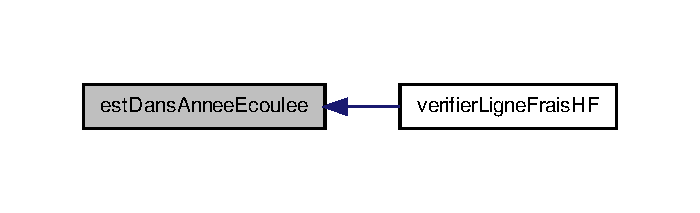
\includegraphics[width=336pt]{__utilitaires_et_gestion_erreurs_8lib_8php_a092454f070d08318790e482128089483_icgraph}
\end{center}
\end{figure}


\hypertarget{__utilitaires_et_gestion_erreurs_8lib_8php_a4f7821728a7b40482111da18fc60603f}{\index{\-\_\-utilitaires\-Et\-Gestion\-Erreurs.\-lib.\-php@{\-\_\-utilitaires\-Et\-Gestion\-Erreurs.\-lib.\-php}!est\-Date@{est\-Date}}
\index{est\-Date@{est\-Date}!_utilitairesEtGestionErreurs.lib.php@{\-\_\-utilitaires\-Et\-Gestion\-Erreurs.\-lib.\-php}}
\subsubsection[{est\-Date}]{\setlength{\rightskip}{0pt plus 5cm}est\-Date (
\begin{DoxyParamCaption}
\item[{}]{\$date}
\end{DoxyParamCaption}
)}}\label{__utilitaires_et_gestion_erreurs_8lib_8php_a4f7821728a7b40482111da18fc60603f}
Vérifie si une chaîne fournie est bien une date valide, au format J\-J/\-M\-M/\-A\-A\-A\-A.

Retrourne true si la chaîne \$date est une date valide, au format J\-J/\-M\-M/\-A\-A\-A\-A, false sinon. 
\begin{DoxyParams}{Paramètres}
{\em string} & date à vérifier \\
\hline
\end{DoxyParams}
\begin{DoxyReturn}{Renvoie}
boolean succès ou échec 
\end{DoxyReturn}


Définition à la ligne 34 du fichier \-\_\-utilitaires\-Et\-Gestion\-Erreurs.\-lib.\-php.



Voici le graphe d'appel pour cette fonction \-:\nopagebreak
\begin{figure}[H]
\begin{center}
\leavevmode
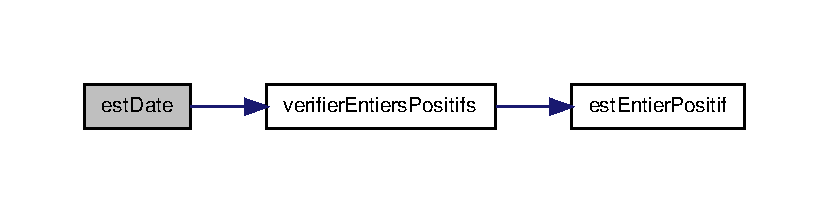
\includegraphics[width=350pt]{__utilitaires_et_gestion_erreurs_8lib_8php_a4f7821728a7b40482111da18fc60603f_cgraph}
\end{center}
\end{figure}




Voici le graphe des appelants de cette fonction \-:\nopagebreak
\begin{figure}[H]
\begin{center}
\leavevmode
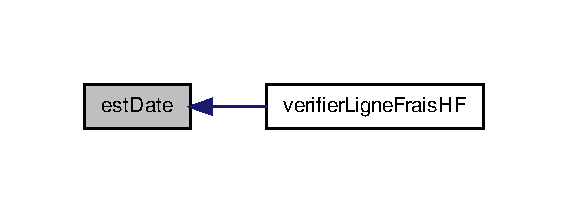
\includegraphics[width=272pt]{__utilitaires_et_gestion_erreurs_8lib_8php_a4f7821728a7b40482111da18fc60603f_icgraph}
\end{center}
\end{figure}


\hypertarget{__utilitaires_et_gestion_erreurs_8lib_8php_a5891ac42bd25b5bb5a9427174f8eb15f}{\index{\-\_\-utilitaires\-Et\-Gestion\-Erreurs.\-lib.\-php@{\-\_\-utilitaires\-Et\-Gestion\-Erreurs.\-lib.\-php}!est\-Entier\-Positif@{est\-Entier\-Positif}}
\index{est\-Entier\-Positif@{est\-Entier\-Positif}!_utilitairesEtGestionErreurs.lib.php@{\-\_\-utilitaires\-Et\-Gestion\-Erreurs.\-lib.\-php}}
\subsubsection[{est\-Entier\-Positif}]{\setlength{\rightskip}{0pt plus 5cm}est\-Entier\-Positif (
\begin{DoxyParamCaption}
\item[{}]{\$valeur}
\end{DoxyParamCaption}
)}}\label{__utilitaires_et_gestion_erreurs_8lib_8php_a5891ac42bd25b5bb5a9427174f8eb15f}
Vérifie si une chaîne fournie est bien numérique entière positive.

Retrourne true si la valeur transmise \$valeur ne contient pas d'autres caractères que des chiffres, false sinon. 
\begin{DoxyParams}{Paramètres}
{\em string} & chaîne à vérifier \\
\hline
\end{DoxyParams}
\begin{DoxyReturn}{Renvoie}
boolean succès ou échec 
\end{DoxyReturn}


Définition à la ligne 95 du fichier \-\_\-utilitaires\-Et\-Gestion\-Erreurs.\-lib.\-php.



Voici le graphe des appelants de cette fonction \-:\nopagebreak
\begin{figure}[H]
\begin{center}
\leavevmode
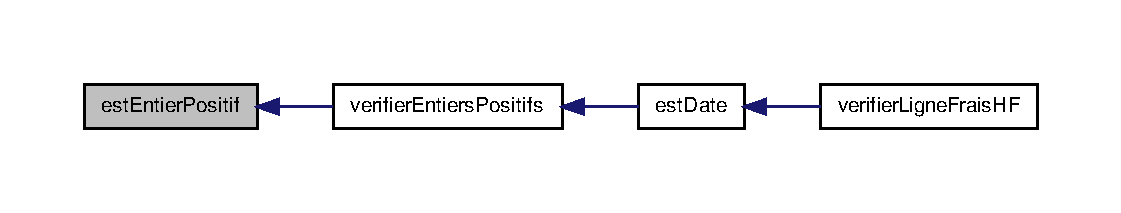
\includegraphics[width=350pt]{__utilitaires_et_gestion_erreurs_8lib_8php_a5891ac42bd25b5bb5a9427174f8eb15f_icgraph}
\end{center}
\end{figure}


\hypertarget{__utilitaires_et_gestion_erreurs_8lib_8php_ad19609774a0abdc797f46e59df5aa55f}{\index{\-\_\-utilitaires\-Et\-Gestion\-Erreurs.\-lib.\-php@{\-\_\-utilitaires\-Et\-Gestion\-Erreurs.\-lib.\-php}!filtrer\-Chaine\-Pour\-Navig@{filtrer\-Chaine\-Pour\-Navig}}
\index{filtrer\-Chaine\-Pour\-Navig@{filtrer\-Chaine\-Pour\-Navig}!_utilitairesEtGestionErreurs.lib.php@{\-\_\-utilitaires\-Et\-Gestion\-Erreurs.\-lib.\-php}}
\subsubsection[{filtrer\-Chaine\-Pour\-Navig}]{\setlength{\rightskip}{0pt plus 5cm}filtrer\-Chaine\-Pour\-Navig (
\begin{DoxyParamCaption}
\item[{}]{\$str}
\end{DoxyParamCaption}
)}}\label{__utilitaires_et_gestion_erreurs_8lib_8php_ad19609774a0abdc797f46e59df5aa55f}
Echappe les caractères considérés spéciaux en H\-T\-M\-L par les entités H\-T\-M\-L correspondantes.

Renvoie une copie de la chaîne \$str à laquelle les caractères considérés spéciaux en H\-T\-M\-L (tq la quote simple, le guillemet double, les chevrons), auront été remplacés par les entités H\-T\-M\-L correspondantes. 
\begin{DoxyParams}[1]{Paramètres}
string & {\em \$str} & chaîne à échapper \\
\hline
\end{DoxyParams}
\begin{DoxyReturn}{Renvoie}
string chaîne échappée 
\end{DoxyReturn}


Définition à la ligne 234 du fichier \-\_\-utilitaires\-Et\-Gestion\-Erreurs.\-lib.\-php.

\hypertarget{__utilitaires_et_gestion_erreurs_8lib_8php_ab4e61487d300e37e058c1fd31c0446a9}{\index{\-\_\-utilitaires\-Et\-Gestion\-Erreurs.\-lib.\-php@{\-\_\-utilitaires\-Et\-Gestion\-Erreurs.\-lib.\-php}!lire\-Donnee@{lire\-Donnee}}
\index{lire\-Donnee@{lire\-Donnee}!_utilitairesEtGestionErreurs.lib.php@{\-\_\-utilitaires\-Et\-Gestion\-Erreurs.\-lib.\-php}}
\subsubsection[{lire\-Donnee}]{\setlength{\rightskip}{0pt plus 5cm}lire\-Donnee (
\begin{DoxyParamCaption}
\item[{}]{\$nom\-Donnee, }
\item[{}]{\$val\-Defaut = {\ttfamily \char`\"{}\char`\"{}}}
\end{DoxyParamCaption}
)}}\label{__utilitaires_et_gestion_erreurs_8lib_8php_ab4e61487d300e37e058c1fd31c0446a9}
Fournit la valeur d'une donnée transmise par la méthode get (url) ou post (corps de la requête H\-T\-T\-P).

Retourne la valeur de la donnée portant le nom \$nom\-Donnee reçue dans l'url ou corps de requête, \$val\-Defaut si aucune donnée de nom \$nom\-Donnee ni dans l'url, ni dans corps. Si le même nom a été transmis à la fois dans l'url et le corps de la requête, c'est la valeur transmise par l'url qui est retournée. 
\begin{DoxyParams}{Paramètres}
{\em string} & nom de la donnée \\
\hline
{\em string} & valeur par défaut \\
\hline
\end{DoxyParams}
\begin{DoxyReturn}{Renvoie}
string valeur de la donnée 
\end{DoxyReturn}


Définition à la ligne 169 du fichier \-\_\-utilitaires\-Et\-Gestion\-Erreurs.\-lib.\-php.

\hypertarget{__utilitaires_et_gestion_erreurs_8lib_8php_ab0070fc1ef4283caa3457dd5b71a86de}{\index{\-\_\-utilitaires\-Et\-Gestion\-Erreurs.\-lib.\-php@{\-\_\-utilitaires\-Et\-Gestion\-Erreurs.\-lib.\-php}!lire\-Donnee\-Post@{lire\-Donnee\-Post}}
\index{lire\-Donnee\-Post@{lire\-Donnee\-Post}!_utilitairesEtGestionErreurs.lib.php@{\-\_\-utilitaires\-Et\-Gestion\-Erreurs.\-lib.\-php}}
\subsubsection[{lire\-Donnee\-Post}]{\setlength{\rightskip}{0pt plus 5cm}lire\-Donnee\-Post (
\begin{DoxyParamCaption}
\item[{}]{\$nom\-Donnee, }
\item[{}]{\$val\-Defaut = {\ttfamily \char`\"{}\char`\"{}}}
\end{DoxyParamCaption}
)}}\label{__utilitaires_et_gestion_erreurs_8lib_8php_ab0070fc1ef4283caa3457dd5b71a86de}
Fournit la valeur d'une donnée transmise par la méthode post (corps de la requête H\-T\-T\-P).

Retourne la valeur de la donnée portant le nom \$nom\-Donnee reçue dans le corps de la requête http, \$val\-Defaut si aucune donnée de nom \$nom\-Donnee dans le corps de requête 
\begin{DoxyParams}{Paramètres}
{\em string} & nom de la donnée \\
\hline
{\em string} & valeur par défaut \\
\hline
\end{DoxyParams}
\begin{DoxyReturn}{Renvoie}
string valeur de la donnée 
\end{DoxyReturn}


Définition à la ligne 146 du fichier \-\_\-utilitaires\-Et\-Gestion\-Erreurs.\-lib.\-php.

\hypertarget{__utilitaires_et_gestion_erreurs_8lib_8php_ad3618b973b51810a2eb97a0493ade9ee}{\index{\-\_\-utilitaires\-Et\-Gestion\-Erreurs.\-lib.\-php@{\-\_\-utilitaires\-Et\-Gestion\-Erreurs.\-lib.\-php}!lire\-Donnee\-Url@{lire\-Donnee\-Url}}
\index{lire\-Donnee\-Url@{lire\-Donnee\-Url}!_utilitairesEtGestionErreurs.lib.php@{\-\_\-utilitaires\-Et\-Gestion\-Erreurs.\-lib.\-php}}
\subsubsection[{lire\-Donnee\-Url}]{\setlength{\rightskip}{0pt plus 5cm}lire\-Donnee\-Url (
\begin{DoxyParamCaption}
\item[{}]{\$nom\-Donnee, }
\item[{}]{\$val\-Defaut = {\ttfamily \char`\"{}\char`\"{}}}
\end{DoxyParamCaption}
)}}\label{__utilitaires_et_gestion_erreurs_8lib_8php_ad3618b973b51810a2eb97a0493ade9ee}
Fournit la valeur d'une donnée transmise par la méthode get (url).

Retourne la valeur de la donnée portant le nom \$nom\-Donnee reçue dans l'url, \$val\-Defaut si aucune donnée de nom \$nom\-Donnee dans l'url 
\begin{DoxyParams}{Paramètres}
{\em string} & nom de la donnée \\
\hline
{\em string} & valeur par défaut \\
\hline
\end{DoxyParams}
\begin{DoxyReturn}{Renvoie}
string valeur de la donnée 
\end{DoxyReturn}


Définition à la ligne 126 du fichier \-\_\-utilitaires\-Et\-Gestion\-Erreurs.\-lib.\-php.

\hypertarget{__utilitaires_et_gestion_erreurs_8lib_8php_a61c228522012792b81b2931ef1ae32ce}{\index{\-\_\-utilitaires\-Et\-Gestion\-Erreurs.\-lib.\-php@{\-\_\-utilitaires\-Et\-Gestion\-Erreurs.\-lib.\-php}!nb\-Erreurs@{nb\-Erreurs}}
\index{nb\-Erreurs@{nb\-Erreurs}!_utilitairesEtGestionErreurs.lib.php@{\-\_\-utilitaires\-Et\-Gestion\-Erreurs.\-lib.\-php}}
\subsubsection[{nb\-Erreurs}]{\setlength{\rightskip}{0pt plus 5cm}nb\-Erreurs (
\begin{DoxyParamCaption}
\item[{}]{\$tab\-Err}
\end{DoxyParamCaption}
)}}\label{__utilitaires_et_gestion_erreurs_8lib_8php_a61c228522012792b81b2931ef1ae32ce}
Retourne le nombre de messages d'erreurs enregistrés.

Retourne le nombre de messages d'erreurs enregistrés dans le tableau \$tab\-Err. 
\begin{DoxyParams}[1]{Paramètres}
array & {\em \$tab\-Err} & tableau des messages d'erreurs \\
\hline
\end{DoxyParams}
\begin{DoxyReturn}{Renvoie}
int nombre de messages d'erreurs 
\end{DoxyReturn}


Définition à la ligne 202 du fichier \-\_\-utilitaires\-Et\-Gestion\-Erreurs.\-lib.\-php.

\hypertarget{__utilitaires_et_gestion_erreurs_8lib_8php_a991bef919e2c370187e9d7eec29f8f50}{\index{\-\_\-utilitaires\-Et\-Gestion\-Erreurs.\-lib.\-php@{\-\_\-utilitaires\-Et\-Gestion\-Erreurs.\-lib.\-php}!obtenir\-Libelle\-Mois@{obtenir\-Libelle\-Mois}}
\index{obtenir\-Libelle\-Mois@{obtenir\-Libelle\-Mois}!_utilitairesEtGestionErreurs.lib.php@{\-\_\-utilitaires\-Et\-Gestion\-Erreurs.\-lib.\-php}}
\subsubsection[{obtenir\-Libelle\-Mois}]{\setlength{\rightskip}{0pt plus 5cm}obtenir\-Libelle\-Mois (
\begin{DoxyParamCaption}
\item[{}]{\$un\-No\-Mois}
\end{DoxyParamCaption}
)}}\label{__utilitaires_et_gestion_erreurs_8lib_8php_a991bef919e2c370187e9d7eec29f8f50}
Fournit le libellé en français correspondant à un numéro de mois.

Fournit le libellé français du mois de numéro \$un\-No\-Mois. Retourne une chaîne vide si le numéro n'est pas compris dans l'intervalle \mbox{[}1,12\mbox{]}. 
\begin{DoxyParams}{Paramètres}
{\em int} & numéro de mois \\
\hline
\end{DoxyParams}
\begin{DoxyReturn}{Renvoie}
string identifiant de connexion 
\end{DoxyReturn}


Définition à la ligne 16 du fichier \-\_\-utilitaires\-Et\-Gestion\-Erreurs.\-lib.\-php.

\hypertarget{__utilitaires_et_gestion_erreurs_8lib_8php_a2ff214e84108237a421875ab1ab3f7fa}{\index{\-\_\-utilitaires\-Et\-Gestion\-Erreurs.\-lib.\-php@{\-\_\-utilitaires\-Et\-Gestion\-Erreurs.\-lib.\-php}!to\-String\-Erreurs@{to\-String\-Erreurs}}
\index{to\-String\-Erreurs@{to\-String\-Erreurs}!_utilitairesEtGestionErreurs.lib.php@{\-\_\-utilitaires\-Et\-Gestion\-Erreurs.\-lib.\-php}}
\subsubsection[{to\-String\-Erreurs}]{\setlength{\rightskip}{0pt plus 5cm}to\-String\-Erreurs (
\begin{DoxyParamCaption}
\item[{}]{\$tab\-Err}
\end{DoxyParamCaption}
)}}\label{__utilitaires_et_gestion_erreurs_8lib_8php_a2ff214e84108237a421875ab1ab3f7fa}
Fournit les messages d'erreurs sous forme d'une liste à puces H\-T\-M\-L.

Retourne le source H\-T\-M\-L, division contenant une liste à puces, d'après les messages d'erreurs contenus dans le tableau des messages d'erreurs \$tab\-Err. 
\begin{DoxyParams}[1]{Paramètres}
array & {\em \$tab\-Err} & tableau des messages d'erreurs \\
\hline
\end{DoxyParams}
\begin{DoxyReturn}{Renvoie}
string source html 
\end{DoxyReturn}


Définition à la ligne 214 du fichier \-\_\-utilitaires\-Et\-Gestion\-Erreurs.\-lib.\-php.

\hypertarget{__utilitaires_et_gestion_erreurs_8lib_8php_a3457b44782886f81a118ee6ae62f9568}{\index{\-\_\-utilitaires\-Et\-Gestion\-Erreurs.\-lib.\-php@{\-\_\-utilitaires\-Et\-Gestion\-Erreurs.\-lib.\-php}!verifier\-Entiers\-Positifs@{verifier\-Entiers\-Positifs}}
\index{verifier\-Entiers\-Positifs@{verifier\-Entiers\-Positifs}!_utilitairesEtGestionErreurs.lib.php@{\-\_\-utilitaires\-Et\-Gestion\-Erreurs.\-lib.\-php}}
\subsubsection[{verifier\-Entiers\-Positifs}]{\setlength{\rightskip}{0pt plus 5cm}verifier\-Entiers\-Positifs (
\begin{DoxyParamCaption}
\item[{}]{\$les\-Valeurs}
\end{DoxyParamCaption}
)}}\label{__utilitaires_et_gestion_erreurs_8lib_8php_a3457b44782886f81a118ee6ae62f9568}
Vérifie que chaque valeur est bien renseignée et numérique entière positive.

Renvoie la valeur booléenne true si toutes les valeurs sont bien renseignées et numériques entières positives. False si l'une d'elles ne l'est pas. 
\begin{DoxyParams}[1]{Paramètres}
array & {\em \$les\-Valeurs} & tableau des valeurs \\
\hline
\end{DoxyParams}
\begin{DoxyReturn}{Renvoie}
booléen succès ou échec 
\end{DoxyReturn}


Définition à la ligne 107 du fichier \-\_\-utilitaires\-Et\-Gestion\-Erreurs.\-lib.\-php.



Voici le graphe d'appel pour cette fonction \-:\nopagebreak
\begin{figure}[H]
\begin{center}
\leavevmode
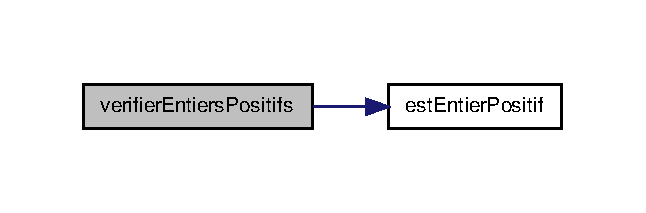
\includegraphics[width=310pt]{__utilitaires_et_gestion_erreurs_8lib_8php_a3457b44782886f81a118ee6ae62f9568_cgraph}
\end{center}
\end{figure}




Voici le graphe des appelants de cette fonction \-:\nopagebreak
\begin{figure}[H]
\begin{center}
\leavevmode
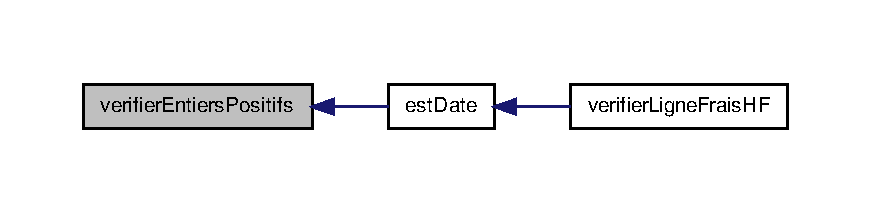
\includegraphics[width=350pt]{__utilitaires_et_gestion_erreurs_8lib_8php_a3457b44782886f81a118ee6ae62f9568_icgraph}
\end{center}
\end{figure}


\hypertarget{__utilitaires_et_gestion_erreurs_8lib_8php_add1850973a586302c7fab9e20bd1dd25}{\index{\-\_\-utilitaires\-Et\-Gestion\-Erreurs.\-lib.\-php@{\-\_\-utilitaires\-Et\-Gestion\-Erreurs.\-lib.\-php}!verifier\-Ligne\-Frais\-H\-F@{verifier\-Ligne\-Frais\-H\-F}}
\index{verifier\-Ligne\-Frais\-H\-F@{verifier\-Ligne\-Frais\-H\-F}!_utilitairesEtGestionErreurs.lib.php@{\-\_\-utilitaires\-Et\-Gestion\-Erreurs.\-lib.\-php}}
\subsubsection[{verifier\-Ligne\-Frais\-H\-F}]{\setlength{\rightskip}{0pt plus 5cm}verifier\-Ligne\-Frais\-H\-F (
\begin{DoxyParamCaption}
\item[{}]{\$date, }
\item[{}]{\$libelle, }
\item[{}]{\$montant, }
\item[{\&}]{\$tab\-Errs}
\end{DoxyParamCaption}
)}}\label{__utilitaires_et_gestion_erreurs_8lib_8php_add1850973a586302c7fab9e20bd1dd25}
Vérifie la validité des données d'une ligne de frais hors forfait.

Renseigne le tableau des messages d'erreurs d'après les erreurs rencontrées sur chaque donnée d'une ligne de frais hors forfait \-: vérifie que chaque donnée est bien renseignée, le montant est numérique positif, la date valide et dans l'année écoulée. 
\begin{DoxyParams}[1]{Paramètres}
array & {\em \$date} & date d'engagement de la ligne de frais H\-F \\
\hline
array & {\em \$libelle} & libellé de la ligne de frais H\-F \\
\hline
array & {\em \$montant} & montant de la ligne de frais H\-F \\
\hline
array & {\em \$tab\-Errs} & tableau des messages d'erreurs passé par référence \\
\hline
\end{DoxyParams}
\begin{DoxyReturn}{Renvoie}
void 
\end{DoxyReturn}


Définition à la ligne 251 du fichier \-\_\-utilitaires\-Et\-Gestion\-Erreurs.\-lib.\-php.



Voici le graphe d'appel pour cette fonction \-:\nopagebreak
\begin{figure}[H]
\begin{center}
\leavevmode
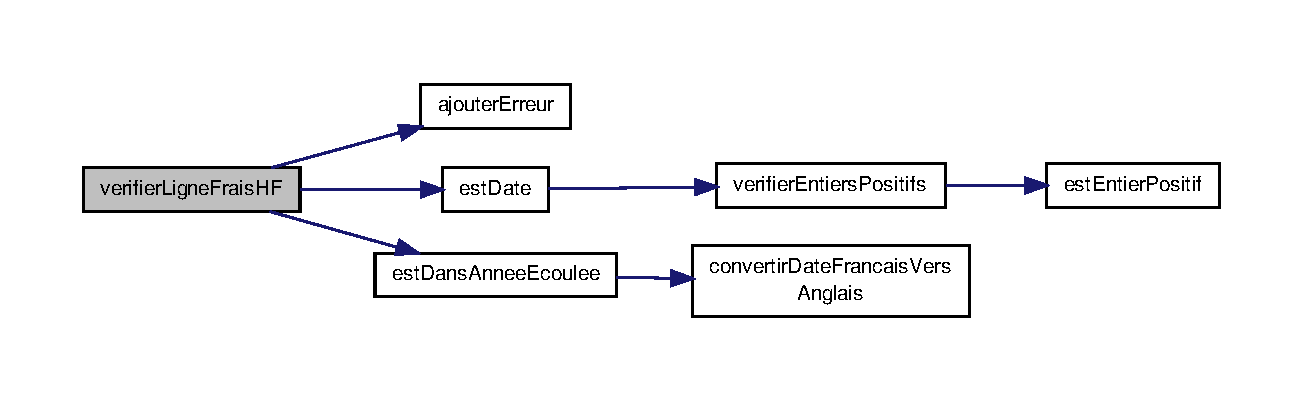
\includegraphics[width=350pt]{__utilitaires_et_gestion_erreurs_8lib_8php_add1850973a586302c7fab9e20bd1dd25_cgraph}
\end{center}
\end{figure}



\hypertarget{fct_8inc_8php}{\section{Référence du fichier /home/trackoen/\-P\-H\-P\-\_\-\-P\-R\-O\-J\-E\-C\-T/\-G\-S\-B\-\_\-\-Appli/include/fct.inc.\-php}
\label{fct_8inc_8php}\index{/home/trackoen/\-P\-H\-P\-\_\-\-P\-R\-O\-J\-E\-C\-T/\-G\-S\-B\-\_\-\-Appli/include/fct.\-inc.\-php@{/home/trackoen/\-P\-H\-P\-\_\-\-P\-R\-O\-J\-E\-C\-T/\-G\-S\-B\-\_\-\-Appli/include/fct.\-inc.\-php}}
}
\subsection*{Fonctions}
\begin{DoxyCompactItemize}
\item 
\hyperlink{fct_8inc_8php_a2acfd2dba761253597a1ab45974a0960}{get\-Les\-Visiteurs} (\$pdo)
\item 
\hyperlink{fct_8inc_8php_a4ddda167f959ca116a8a3e6eeb90fa9e}{get\-Les\-Fiches\-Frais} (\$pdo)
\item 
\hyperlink{fct_8inc_8php_a6308942d3ba830a09e7e94ae7711e484}{get\-Les\-Id\-Frais\-Forfait} (\$pdo)
\item 
\hyperlink{fct_8inc_8php_a24de2eaeae5f67c359ec963e032dc070}{get\-Dernier\-Mois} (\$pdo, \$id\-Visiteur)
\item 
\hyperlink{fct_8inc_8php_a645aa8a245cbeb2d0d167fcc942b9b5c}{get\-Mois\-Suivant} (\$mois)
\item 
\hyperlink{fct_8inc_8php_aeeb91507878426d6313448a6bd1cad7c}{get\-Mois\-Precedent} (\$mois)
\item 
\hyperlink{fct_8inc_8php_aaa271411c3446ad3c57a1429136fc1bf}{creation\-Fiches\-Frais} (\$pdo)
\item 
\hyperlink{fct_8inc_8php_a15cec1f321241d0de7115e96cfccf67f}{creation\-Frais\-Forfait} (\$pdo)
\item 
\hyperlink{fct_8inc_8php_ae0eddc9c28d0ed7a68aa28fa98a6f214}{get\-Des\-Frais\-Hors\-Forfait} ()
\item 
\hyperlink{fct_8inc_8php_ad1a28b1457da19e4210dfa8869d1c874}{update\-Mdp\-Visiteur} (\$pdo)
\item 
\hyperlink{fct_8inc_8php_ad980a8fa84e6aee8092ec6525bf1cd5a}{creation\-Frais\-Hors\-Forfait} (\$pdo)
\item 
\hyperlink{fct_8inc_8php_ac6b26dbc90d7a5ec71b0585ee0786a41}{get\-Mois} (\$date)
\item 
\hyperlink{fct_8inc_8php_a737fc7684b15055a48683ee1f6683b5b}{maj\-Fiche\-Frais} (\$pdo)
\end{DoxyCompactItemize}


\subsection{Documentation des fonctions}
\hypertarget{fct_8inc_8php_aaa271411c3446ad3c57a1429136fc1bf}{\index{fct.\-inc.\-php@{fct.\-inc.\-php}!creation\-Fiches\-Frais@{creation\-Fiches\-Frais}}
\index{creation\-Fiches\-Frais@{creation\-Fiches\-Frais}!fct.inc.php@{fct.\-inc.\-php}}
\subsubsection[{creation\-Fiches\-Frais}]{\setlength{\rightskip}{0pt plus 5cm}creation\-Fiches\-Frais (
\begin{DoxyParamCaption}
\item[{}]{\$pdo}
\end{DoxyParamCaption}
)}}\label{fct_8inc_8php_aaa271411c3446ad3c57a1429136fc1bf}


Définition à la ligne 61 du fichier fct.\-inc.\-php.



Voici le graphe d'appel pour cette fonction \-:\nopagebreak
\begin{figure}[H]
\begin{center}
\leavevmode
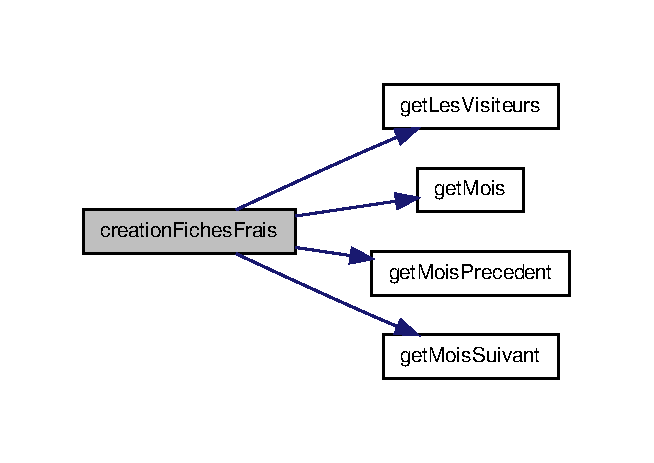
\includegraphics[width=314pt]{fct_8inc_8php_aaa271411c3446ad3c57a1429136fc1bf_cgraph}
\end{center}
\end{figure}


\hypertarget{fct_8inc_8php_a15cec1f321241d0de7115e96cfccf67f}{\index{fct.\-inc.\-php@{fct.\-inc.\-php}!creation\-Frais\-Forfait@{creation\-Frais\-Forfait}}
\index{creation\-Frais\-Forfait@{creation\-Frais\-Forfait}!fct.inc.php@{fct.\-inc.\-php}}
\subsubsection[{creation\-Frais\-Forfait}]{\setlength{\rightskip}{0pt plus 5cm}creation\-Frais\-Forfait (
\begin{DoxyParamCaption}
\item[{}]{\$pdo}
\end{DoxyParamCaption}
)}}\label{fct_8inc_8php_a15cec1f321241d0de7115e96cfccf67f}


Définition à la ligne 104 du fichier fct.\-inc.\-php.



Voici le graphe d'appel pour cette fonction \-:\nopagebreak
\begin{figure}[H]
\begin{center}
\leavevmode
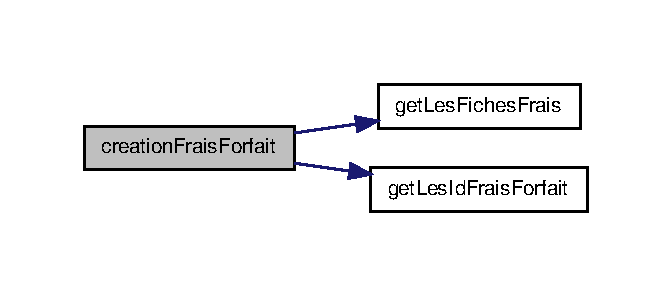
\includegraphics[width=322pt]{fct_8inc_8php_a15cec1f321241d0de7115e96cfccf67f_cgraph}
\end{center}
\end{figure}


\hypertarget{fct_8inc_8php_ad980a8fa84e6aee8092ec6525bf1cd5a}{\index{fct.\-inc.\-php@{fct.\-inc.\-php}!creation\-Frais\-Hors\-Forfait@{creation\-Frais\-Hors\-Forfait}}
\index{creation\-Frais\-Hors\-Forfait@{creation\-Frais\-Hors\-Forfait}!fct.inc.php@{fct.\-inc.\-php}}
\subsubsection[{creation\-Frais\-Hors\-Forfait}]{\setlength{\rightskip}{0pt plus 5cm}creation\-Frais\-Hors\-Forfait (
\begin{DoxyParamCaption}
\item[{}]{\$pdo}
\end{DoxyParamCaption}
)}}\label{fct_8inc_8php_ad980a8fa84e6aee8092ec6525bf1cd5a}


Définition à la ligne 202 du fichier fct.\-inc.\-php.



Voici le graphe d'appel pour cette fonction \-:\nopagebreak
\begin{figure}[H]
\begin{center}
\leavevmode
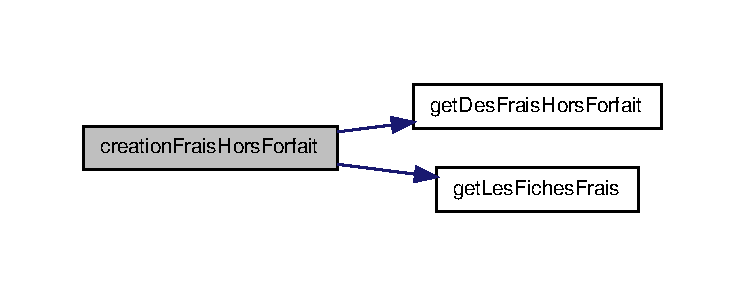
\includegraphics[width=350pt]{fct_8inc_8php_ad980a8fa84e6aee8092ec6525bf1cd5a_cgraph}
\end{center}
\end{figure}


\hypertarget{fct_8inc_8php_a24de2eaeae5f67c359ec963e032dc070}{\index{fct.\-inc.\-php@{fct.\-inc.\-php}!get\-Dernier\-Mois@{get\-Dernier\-Mois}}
\index{get\-Dernier\-Mois@{get\-Dernier\-Mois}!fct.inc.php@{fct.\-inc.\-php}}
\subsubsection[{get\-Dernier\-Mois}]{\setlength{\rightskip}{0pt plus 5cm}get\-Dernier\-Mois (
\begin{DoxyParamCaption}
\item[{}]{\$pdo, }
\item[{}]{\$id\-Visiteur}
\end{DoxyParamCaption}
)}}\label{fct_8inc_8php_a24de2eaeae5f67c359ec963e032dc070}


Définition à la ligne 24 du fichier fct.\-inc.\-php.



Voici le graphe des appelants de cette fonction \-:\nopagebreak
\begin{figure}[H]
\begin{center}
\leavevmode
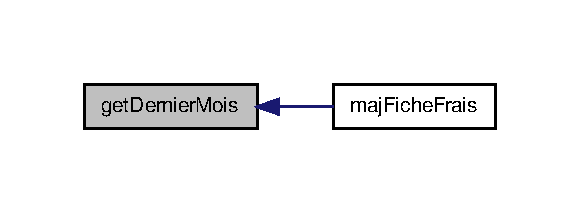
\includegraphics[width=278pt]{fct_8inc_8php_a24de2eaeae5f67c359ec963e032dc070_icgraph}
\end{center}
\end{figure}


\hypertarget{fct_8inc_8php_ae0eddc9c28d0ed7a68aa28fa98a6f214}{\index{fct.\-inc.\-php@{fct.\-inc.\-php}!get\-Des\-Frais\-Hors\-Forfait@{get\-Des\-Frais\-Hors\-Forfait}}
\index{get\-Des\-Frais\-Hors\-Forfait@{get\-Des\-Frais\-Hors\-Forfait}!fct.inc.php@{fct.\-inc.\-php}}
\subsubsection[{get\-Des\-Frais\-Hors\-Forfait}]{\setlength{\rightskip}{0pt plus 5cm}get\-Des\-Frais\-Hors\-Forfait (
\begin{DoxyParamCaption}
{}
\end{DoxyParamCaption}
)}}\label{fct_8inc_8php_ae0eddc9c28d0ed7a68aa28fa98a6f214}


Définition à la ligne 130 du fichier fct.\-inc.\-php.



Voici le graphe des appelants de cette fonction \-:\nopagebreak
\begin{figure}[H]
\begin{center}
\leavevmode
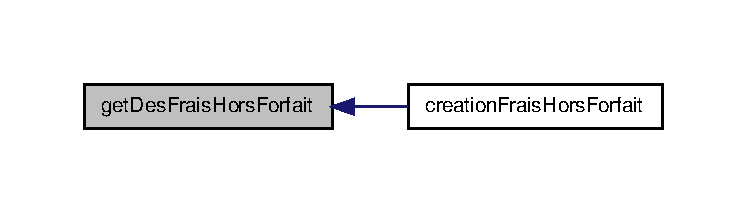
\includegraphics[width=350pt]{fct_8inc_8php_ae0eddc9c28d0ed7a68aa28fa98a6f214_icgraph}
\end{center}
\end{figure}


\hypertarget{fct_8inc_8php_a4ddda167f959ca116a8a3e6eeb90fa9e}{\index{fct.\-inc.\-php@{fct.\-inc.\-php}!get\-Les\-Fiches\-Frais@{get\-Les\-Fiches\-Frais}}
\index{get\-Les\-Fiches\-Frais@{get\-Les\-Fiches\-Frais}!fct.inc.php@{fct.\-inc.\-php}}
\subsubsection[{get\-Les\-Fiches\-Frais}]{\setlength{\rightskip}{0pt plus 5cm}get\-Les\-Fiches\-Frais (
\begin{DoxyParamCaption}
\item[{}]{\$pdo}
\end{DoxyParamCaption}
)}}\label{fct_8inc_8php_a4ddda167f959ca116a8a3e6eeb90fa9e}


Définition à la ligne 10 du fichier fct.\-inc.\-php.



Voici le graphe des appelants de cette fonction \-:\nopagebreak
\begin{figure}[H]
\begin{center}
\leavevmode
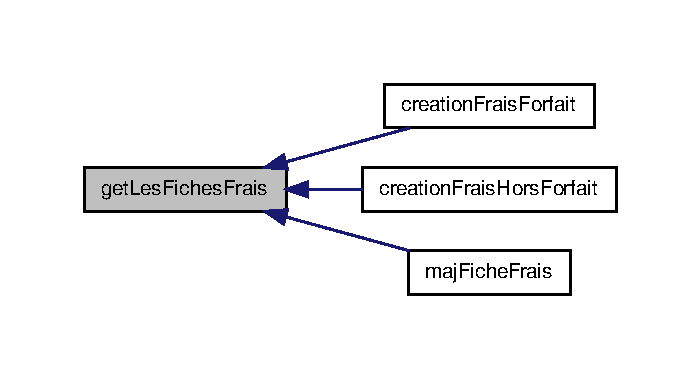
\includegraphics[width=336pt]{fct_8inc_8php_a4ddda167f959ca116a8a3e6eeb90fa9e_icgraph}
\end{center}
\end{figure}


\hypertarget{fct_8inc_8php_a6308942d3ba830a09e7e94ae7711e484}{\index{fct.\-inc.\-php@{fct.\-inc.\-php}!get\-Les\-Id\-Frais\-Forfait@{get\-Les\-Id\-Frais\-Forfait}}
\index{get\-Les\-Id\-Frais\-Forfait@{get\-Les\-Id\-Frais\-Forfait}!fct.inc.php@{fct.\-inc.\-php}}
\subsubsection[{get\-Les\-Id\-Frais\-Forfait}]{\setlength{\rightskip}{0pt plus 5cm}get\-Les\-Id\-Frais\-Forfait (
\begin{DoxyParamCaption}
\item[{}]{\$pdo}
\end{DoxyParamCaption}
)}}\label{fct_8inc_8php_a6308942d3ba830a09e7e94ae7711e484}


Définition à la ligne 17 du fichier fct.\-inc.\-php.



Voici le graphe des appelants de cette fonction \-:\nopagebreak
\begin{figure}[H]
\begin{center}
\leavevmode
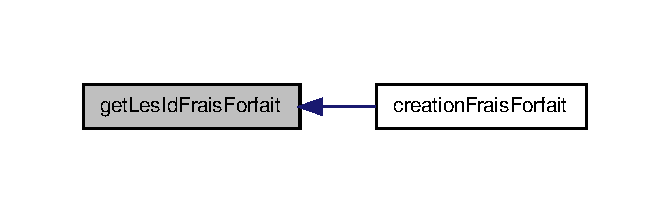
\includegraphics[width=322pt]{fct_8inc_8php_a6308942d3ba830a09e7e94ae7711e484_icgraph}
\end{center}
\end{figure}


\hypertarget{fct_8inc_8php_a2acfd2dba761253597a1ab45974a0960}{\index{fct.\-inc.\-php@{fct.\-inc.\-php}!get\-Les\-Visiteurs@{get\-Les\-Visiteurs}}
\index{get\-Les\-Visiteurs@{get\-Les\-Visiteurs}!fct.inc.php@{fct.\-inc.\-php}}
\subsubsection[{get\-Les\-Visiteurs}]{\setlength{\rightskip}{0pt plus 5cm}get\-Les\-Visiteurs (
\begin{DoxyParamCaption}
\item[{}]{\$pdo}
\end{DoxyParamCaption}
)}}\label{fct_8inc_8php_a2acfd2dba761253597a1ab45974a0960}


Définition à la ligne 3 du fichier fct.\-inc.\-php.



Voici le graphe des appelants de cette fonction \-:\nopagebreak
\begin{figure}[H]
\begin{center}
\leavevmode
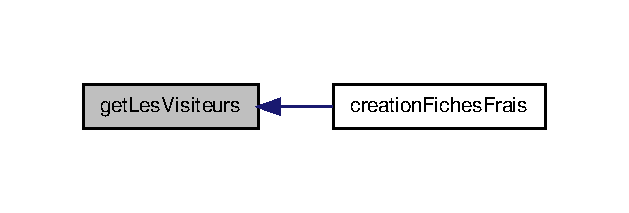
\includegraphics[width=302pt]{fct_8inc_8php_a2acfd2dba761253597a1ab45974a0960_icgraph}
\end{center}
\end{figure}


\hypertarget{fct_8inc_8php_ac6b26dbc90d7a5ec71b0585ee0786a41}{\index{fct.\-inc.\-php@{fct.\-inc.\-php}!get\-Mois@{get\-Mois}}
\index{get\-Mois@{get\-Mois}!fct.inc.php@{fct.\-inc.\-php}}
\subsubsection[{get\-Mois}]{\setlength{\rightskip}{0pt plus 5cm}get\-Mois (
\begin{DoxyParamCaption}
\item[{}]{\$date}
\end{DoxyParamCaption}
)}}\label{fct_8inc_8php_ac6b26dbc90d7a5ec71b0585ee0786a41}


Définition à la ligne 234 du fichier fct.\-inc.\-php.



Voici le graphe des appelants de cette fonction \-:\nopagebreak
\begin{figure}[H]
\begin{center}
\leavevmode
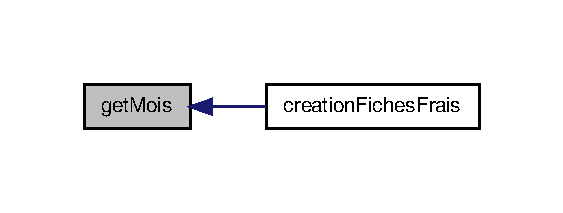
\includegraphics[width=270pt]{fct_8inc_8php_ac6b26dbc90d7a5ec71b0585ee0786a41_icgraph}
\end{center}
\end{figure}


\hypertarget{fct_8inc_8php_aeeb91507878426d6313448a6bd1cad7c}{\index{fct.\-inc.\-php@{fct.\-inc.\-php}!get\-Mois\-Precedent@{get\-Mois\-Precedent}}
\index{get\-Mois\-Precedent@{get\-Mois\-Precedent}!fct.inc.php@{fct.\-inc.\-php}}
\subsubsection[{get\-Mois\-Precedent}]{\setlength{\rightskip}{0pt plus 5cm}get\-Mois\-Precedent (
\begin{DoxyParamCaption}
\item[{}]{\$mois}
\end{DoxyParamCaption}
)}}\label{fct_8inc_8php_aeeb91507878426d6313448a6bd1cad7c}


Définition à la ligne 47 du fichier fct.\-inc.\-php.



Voici le graphe des appelants de cette fonction \-:\nopagebreak
\begin{figure}[H]
\begin{center}
\leavevmode
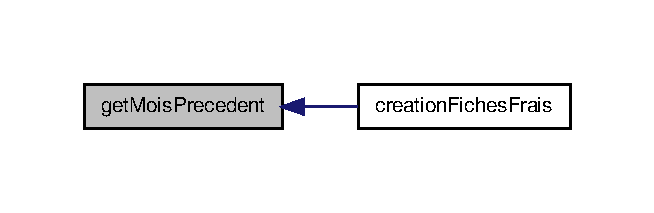
\includegraphics[width=314pt]{fct_8inc_8php_aeeb91507878426d6313448a6bd1cad7c_icgraph}
\end{center}
\end{figure}


\hypertarget{fct_8inc_8php_a645aa8a245cbeb2d0d167fcc942b9b5c}{\index{fct.\-inc.\-php@{fct.\-inc.\-php}!get\-Mois\-Suivant@{get\-Mois\-Suivant}}
\index{get\-Mois\-Suivant@{get\-Mois\-Suivant}!fct.inc.php@{fct.\-inc.\-php}}
\subsubsection[{get\-Mois\-Suivant}]{\setlength{\rightskip}{0pt plus 5cm}get\-Mois\-Suivant (
\begin{DoxyParamCaption}
\item[{}]{\$mois}
\end{DoxyParamCaption}
)}}\label{fct_8inc_8php_a645aa8a245cbeb2d0d167fcc942b9b5c}


Définition à la ligne 32 du fichier fct.\-inc.\-php.



Voici le graphe des appelants de cette fonction \-:\nopagebreak
\begin{figure}[H]
\begin{center}
\leavevmode
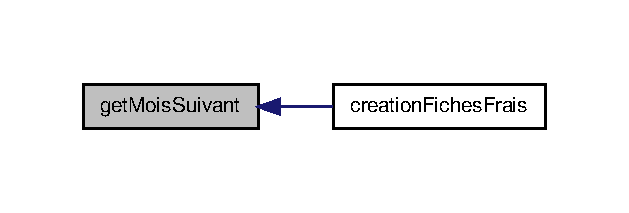
\includegraphics[width=302pt]{fct_8inc_8php_a645aa8a245cbeb2d0d167fcc942b9b5c_icgraph}
\end{center}
\end{figure}


\hypertarget{fct_8inc_8php_a737fc7684b15055a48683ee1f6683b5b}{\index{fct.\-inc.\-php@{fct.\-inc.\-php}!maj\-Fiche\-Frais@{maj\-Fiche\-Frais}}
\index{maj\-Fiche\-Frais@{maj\-Fiche\-Frais}!fct.inc.php@{fct.\-inc.\-php}}
\subsubsection[{maj\-Fiche\-Frais}]{\setlength{\rightskip}{0pt plus 5cm}maj\-Fiche\-Frais (
\begin{DoxyParamCaption}
\item[{}]{\$pdo}
\end{DoxyParamCaption}
)}}\label{fct_8inc_8php_a737fc7684b15055a48683ee1f6683b5b}


Définition à la ligne 241 du fichier fct.\-inc.\-php.



Voici le graphe d'appel pour cette fonction \-:\nopagebreak
\begin{figure}[H]
\begin{center}
\leavevmode
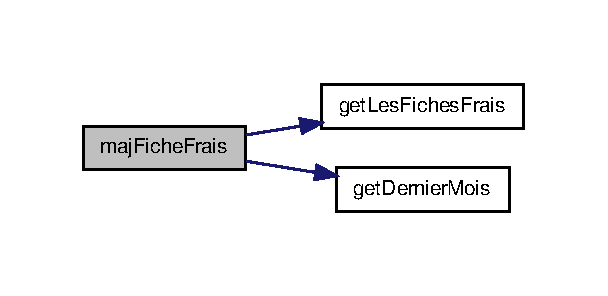
\includegraphics[width=292pt]{fct_8inc_8php_a737fc7684b15055a48683ee1f6683b5b_cgraph}
\end{center}
\end{figure}


\hypertarget{fct_8inc_8php_ad1a28b1457da19e4210dfa8869d1c874}{\index{fct.\-inc.\-php@{fct.\-inc.\-php}!update\-Mdp\-Visiteur@{update\-Mdp\-Visiteur}}
\index{update\-Mdp\-Visiteur@{update\-Mdp\-Visiteur}!fct.inc.php@{fct.\-inc.\-php}}
\subsubsection[{update\-Mdp\-Visiteur}]{\setlength{\rightskip}{0pt plus 5cm}update\-Mdp\-Visiteur (
\begin{DoxyParamCaption}
\item[{}]{\$pdo}
\end{DoxyParamCaption}
)}}\label{fct_8inc_8php_ad1a28b1457da19e4210dfa8869d1c874}


Définition à la ligne 180 du fichier fct.\-inc.\-php.


\hypertarget{maj_g_s_b__main_8php}{\section{Référence du fichier /home/trackoen/\-P\-H\-P\-\_\-\-P\-R\-O\-J\-E\-C\-T/\-G\-S\-B\-\_\-\-Appli/maj\-G\-S\-B\-\_\-main.php}
\label{maj_g_s_b__main_8php}\index{/home/trackoen/\-P\-H\-P\-\_\-\-P\-R\-O\-J\-E\-C\-T/\-G\-S\-B\-\_\-\-Appli/maj\-G\-S\-B\-\_\-main.\-php@{/home/trackoen/\-P\-H\-P\-\_\-\-P\-R\-O\-J\-E\-C\-T/\-G\-S\-B\-\_\-\-Appli/maj\-G\-S\-B\-\_\-main.\-php}}
}
\subsection*{Variables}
\begin{DoxyCompactItemize}
\item 
\hyperlink{maj_g_s_b__main_8php_a4ffb9d7258acf24e1ff550bceba60ed2}{\$serveur} = 'mysql\-:host=localhost'
\item 
\hyperlink{maj_g_s_b__main_8php_a94f91e878bce0991e2cd595c5dd79b3f}{\$bdd} = 'dbname=gsb\-\_\-frais'
\item 
\hyperlink{maj_g_s_b__main_8php_a598ca4e71b15a1313ec95f0df1027ca5}{\$user} = 'root'
\item 
\hyperlink{maj_g_s_b__main_8php_a8a65334de2f0d486a42b02ecf82fe8fb}{\$mdp} = 'lechien'
\end{DoxyCompactItemize}


\subsection{Documentation des variables}
\hypertarget{maj_g_s_b__main_8php_a94f91e878bce0991e2cd595c5dd79b3f}{\index{maj\-G\-S\-B\-\_\-main.\-php@{maj\-G\-S\-B\-\_\-main.\-php}!\$bdd@{\$bdd}}
\index{\$bdd@{\$bdd}!majGSB_main.php@{maj\-G\-S\-B\-\_\-main.\-php}}
\subsubsection[{\$bdd}]{\setlength{\rightskip}{0pt plus 5cm}\$bdd = 'dbname=gsb\-\_\-frais'}}\label{maj_g_s_b__main_8php_a94f91e878bce0991e2cd595c5dd79b3f}


Définition à la ligne 9 du fichier maj\-G\-S\-B\-\_\-main.\-php.

\hypertarget{maj_g_s_b__main_8php_a8a65334de2f0d486a42b02ecf82fe8fb}{\index{maj\-G\-S\-B\-\_\-main.\-php@{maj\-G\-S\-B\-\_\-main.\-php}!\$mdp@{\$mdp}}
\index{\$mdp@{\$mdp}!majGSB_main.php@{maj\-G\-S\-B\-\_\-main.\-php}}
\subsubsection[{\$mdp}]{\setlength{\rightskip}{0pt plus 5cm}\$mdp = 'lechien'}}\label{maj_g_s_b__main_8php_a8a65334de2f0d486a42b02ecf82fe8fb}


Définition à la ligne 11 du fichier maj\-G\-S\-B\-\_\-main.\-php.

\hypertarget{maj_g_s_b__main_8php_a4ffb9d7258acf24e1ff550bceba60ed2}{\index{maj\-G\-S\-B\-\_\-main.\-php@{maj\-G\-S\-B\-\_\-main.\-php}!\$serveur@{\$serveur}}
\index{\$serveur@{\$serveur}!majGSB_main.php@{maj\-G\-S\-B\-\_\-main.\-php}}
\subsubsection[{\$serveur}]{\setlength{\rightskip}{0pt plus 5cm}\$serveur = 'mysql\-:host=localhost'}}\label{maj_g_s_b__main_8php_a4ffb9d7258acf24e1ff550bceba60ed2}


Définition à la ligne 8 du fichier maj\-G\-S\-B\-\_\-main.\-php.

\hypertarget{maj_g_s_b__main_8php_a598ca4e71b15a1313ec95f0df1027ca5}{\index{maj\-G\-S\-B\-\_\-main.\-php@{maj\-G\-S\-B\-\_\-main.\-php}!\$user@{\$user}}
\index{\$user@{\$user}!majGSB_main.php@{maj\-G\-S\-B\-\_\-main.\-php}}
\subsubsection[{\$user}]{\setlength{\rightskip}{0pt plus 5cm}\$user = 'root'}}\label{maj_g_s_b__main_8php_a598ca4e71b15a1313ec95f0df1027ca5}


Définition à la ligne 10 du fichier maj\-G\-S\-B\-\_\-main.\-php.


\printindex
\end{document}
